\documentclass{article}

\usepackage[final]{../NeurIPS-Dataset-Styles/neurips_data_2024/neurips_data_2024}
\usepackage[utf8]{inputenc}
\usepackage[T1]{fontenc}
\usepackage{graphicx}
\usepackage{booktabs}
\usepackage{amsmath}
\usepackage{microtype}
\usepackage{xcolor}
\usepackage{url}
\usepackage{hyperref}
\usepackage{float}
\usepackage{placeins}

\title{Temporal Patterns in New York City Taxi Trips:\\
Data Cleaning, Feature Generation and Exploration}

\author{%
  Msesenyane Makhongela \\
  School of Computer Science and Applied Mathematics \\
  University of the Witwatersrand \\
  Johannesburg, South Africa
}

\begin{document}

\maketitle

\begin{abstract}
This report explores temporal patterns in the New York City Taxi Trip Duration
training sample. The data contain 1,458,644 trips recorded between January and
June 2016. Implausible durations, distances, speeds, coordinates and passenger
counts were removed before analysis. The cleaning process retained 1,443,535
trips, or 98.96\% of the original sample. Friday had the highest average daily
trip count. Weekday demand was concentrated around the evening commute, while
weekend activity shifted towards late-night hours. Memorial Day produced the
largest holiday reduction, whereas Valentine's Day was busier than a typical
Sunday. Average trip speed was highest at 05:00 and lowest during the congested
daytime period.
\end{abstract}

\section{Introduction}

The New York City Taxi Trip Duration dataset contains pickup and drop-off
times, coordinates, passenger counts and trip durations for trips recorded
between 1 January and 30 June 2016 \cite{nyctaxi}. This report addresses three
tasks. First, it identifies and removes implausible observations. Second, it
generates distance, day-of-week and average-speed features. Third, it uses the
cleaned data to examine daily, hourly, weekday, weekend and holiday patterns.

All temporal results use pickup time. Trip counts refer to the Kaggle training
sample rather than every taxi trip completed in New York City. They are
therefore treated as a consistent measure of activity within the sample.

\section{Data cleaning}

The dataset contained 1,458,644 rows and no missing values. However, several
values were not plausible. The maximum recorded duration was approximately
40.8 days, the maximum straight-line distance was 1,240.9 km, and the maximum
implied average speed was 9,274.8 km/h. Some coordinates were also far outside
New York City, while 65 trips had passenger counts outside the valid range of
one to six.

Distance was calculated using the Haversine formula:

\begin{equation}
  d = 2R\arcsin\left(\sqrt{
  \sin^2\left(\frac{\Delta\phi}{2}\right) +
  \cos(\phi_1)\cos(\phi_2)
  \sin^2\left(\frac{\Delta\lambda}{2}\right)}\right),
\end{equation}

where $R=6371.0088$ km, $\phi$ is latitude and $\lambda$ is longitude. This
gives straight-line distance rather than road distance, but it is sufficient
for detecting major coordinate and speed errors.

Table~\ref{tab:cleaning} summarises the cleaning rules. The limits were kept
broad so that unusual but credible trips remained in the sample. A duration
below 30 seconds is unlikely to represent a completed passenger trip, while a
duration above four hours is more likely to indicate a timestamp or meter
error. Distances below 50 metres make speed unreliable, and distances above
100 km are extreme for this setting. An average speed above 120 km/h is not
credible for a taxi travelling through New York. The coordinate boundary
includes Manhattan, JFK, LaGuardia and Newark while excluding distant points.

\begin{table}[H]
  \caption{Cleaning rules and the number of trips flagged}
  \label{tab:cleaning}
  \centering
  \small
  \begin{tabular}{lr}
    \toprule
    Criterion & Trips flagged \\
    \midrule
    Duration outside 30 seconds to 4 hours & 6,859 \\
    Distance outside 0.05 to 100 km & 11,348 \\
    Average speed above 120 km/h & 136 \\
    Pickup or drop-off outside the NYC metro box & 998 \\
    Passenger count outside 1 to 6 & 65 \\
    \bottomrule
  \end{tabular}
\end{table}

The rules overlap, so their individual counts cannot be added. A trip was
removed if it failed at least one rule. In total, 15,109 trips were removed,
leaving 1,443,535 trips. This is a reduction of only 1.04\%, so the later
patterns are not produced by aggressive trimming. Figure~\ref{fig:cleaning}
shows the raw distributions and the selected boundaries.

\begin{figure}[H]
  \centering
  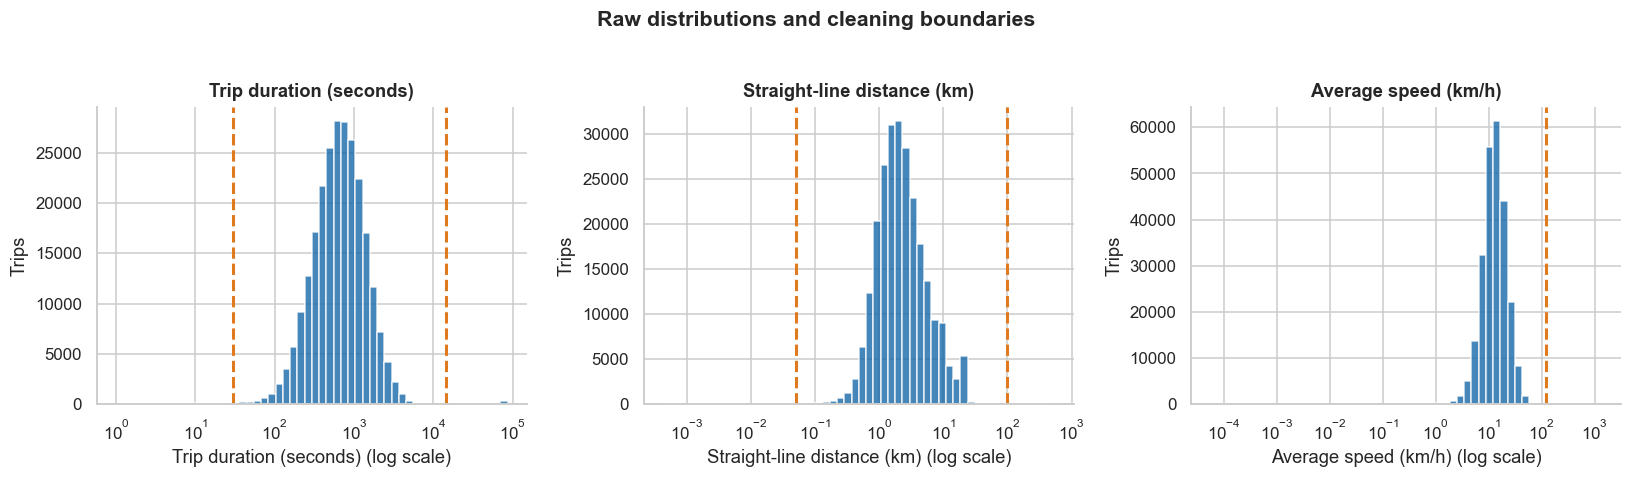
\includegraphics[width=\linewidth]{figures/cleaning_diagnostics.png}
  \caption{Raw duration, straight-line distance and average-speed
  distributions. The horizontal axes are logarithmic and dashed lines show
  the cleaning boundaries.}
  \label{fig:cleaning}
\end{figure}

\section{Feature generation}

Three required features were generated. Trip distance was calculated in
kilometres using the Haversine formula. Day of week was extracted from pickup
time and stored as an ordered category from Monday to Sunday. Average speed was
calculated as

\begin{equation}
  \text{average speed (km/h)} =
  \frac{\text{distance (km)}}{\text{trip duration (seconds)} / 3600}.
\end{equation}

Pickup date, hour, weekday number and a weekday/weekend indicator were also
created. These additional fields allowed each temporal comparison to be
performed directly and kept the weekday order consistent across tables and
figures.

\section{Time-based analysis}

\subsection{Most popular day of the week}

Friday was the most popular day, with an average of 8,507.5 trips per day.
Saturday was close behind with 8,406.9 trips. The six-month period contains 26
occurrences of every weekday, so total counts and average daily counts produce
the same ranking. The average is reported because it is easier to interpret
and remains appropriate for periods with unequal weekday frequencies.

\begin{figure}[H]
  \centering
  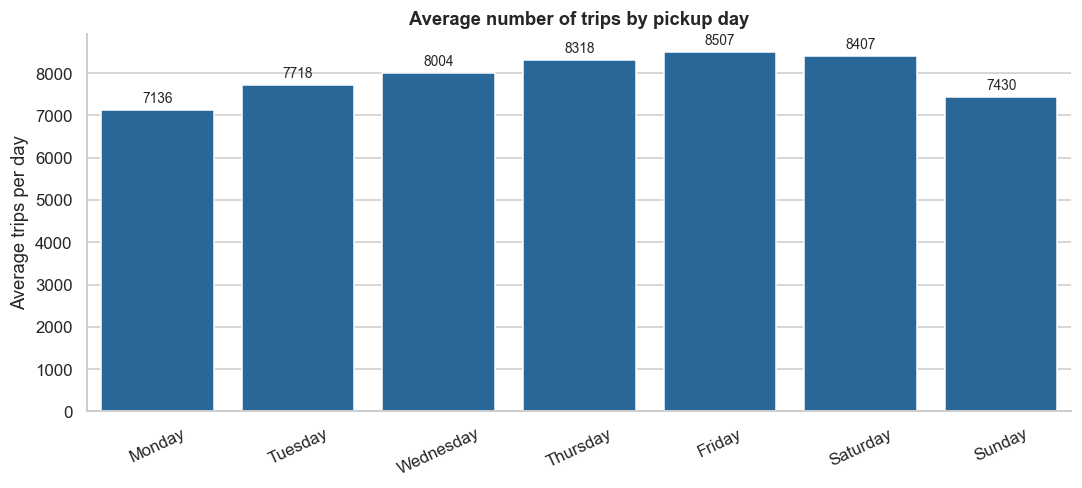
\includegraphics[width=0.88\linewidth]{figures/weekday_popularity.png}
  \caption{Average number of trips by pickup day. Friday recorded the highest
  daily average, followed by Saturday.}
  \label{fig:weekday}
\end{figure}

\subsection{Most popular hour on each day}

Figure~\ref{fig:heatmap} shows the share of each weekday's trips occurring in
each hour. Monday and Tuesday peaked at 18:00, Wednesday at 19:00, Thursday at
21:00, Friday at 19:00, Saturday at 23:00 and Sunday at 00:00.

\begin{figure}[H]
  \centering
  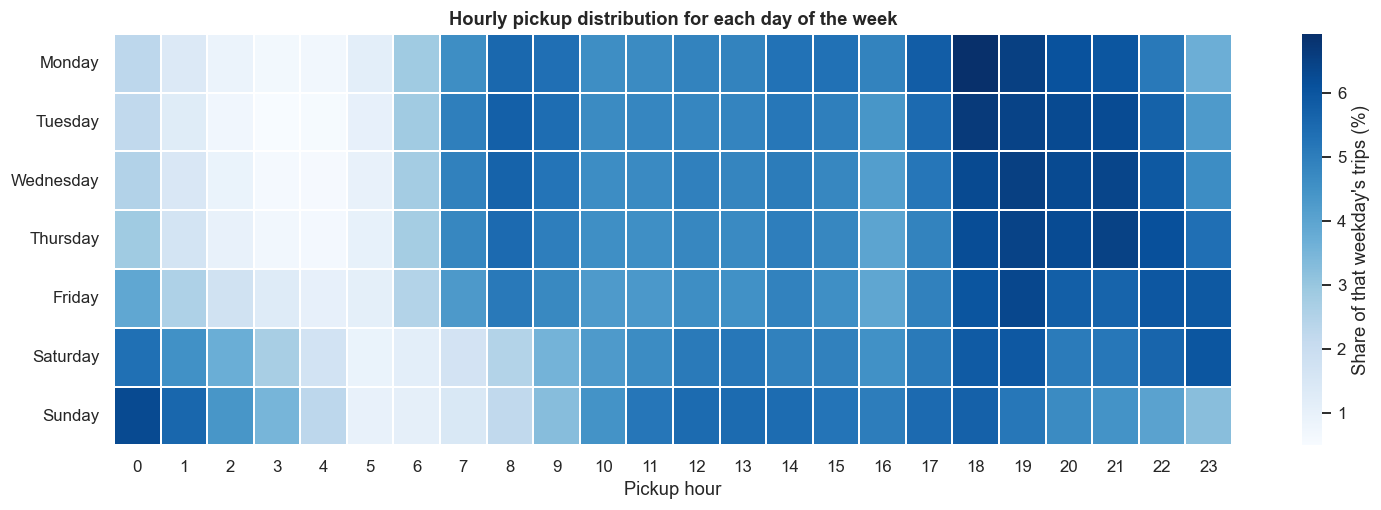
\includegraphics[width=\linewidth]{figures/weekday_hour_heatmap.png}
  \caption{Hourly pickup distribution for each day of the week. Colour shows
  the percentage of that weekday's trips occurring in each hour.}
  \label{fig:heatmap}
\end{figure}

The Monday-to-Wednesday peaks are consistent with evening commuting and
after-work activity. Thursday and Friday remain busy later, while the Saturday
and Sunday midnight peaks are consistent with nightlife trips crossing into
the early morning. These are plausible explanations rather than confirmed trip
purposes because the dataset does not record why each passenger travelled.

\subsection{Weekdays and weekends}

Figure~\ref{fig:daytype} compares average hourly counts per day. Weekdays show
clear morning and evening commuter patterns. Weekend activity begins later in
the morning and is stronger between 22:00 and 01:00. Despite these different
shapes, the average daily volumes are almost identical: 7,936.7 trips on a
weekday and 7,918.5 on a weekend day.

\begin{figure}[H]
  \centering
  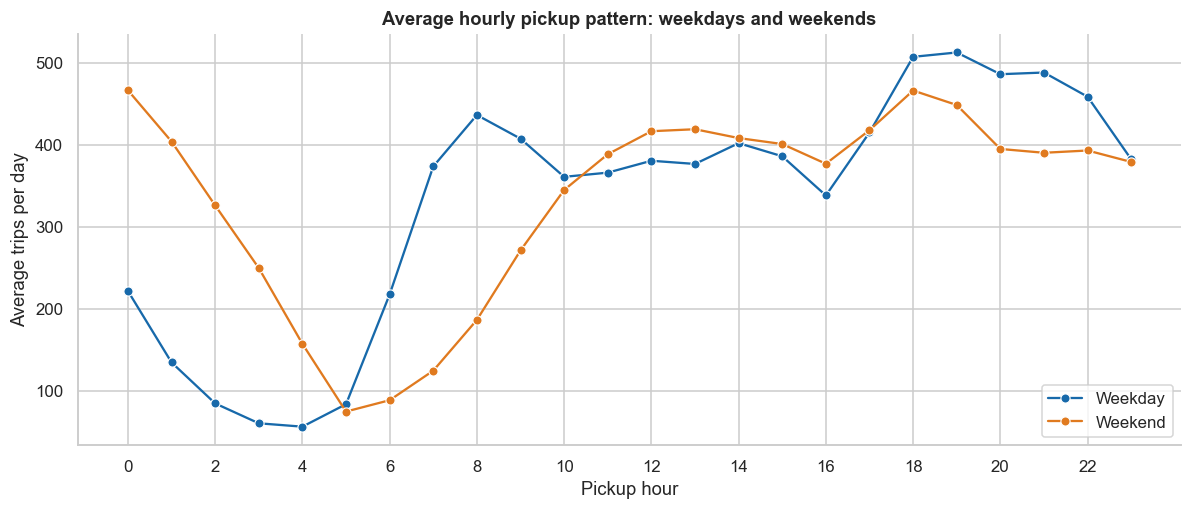
\includegraphics[width=0.9\linewidth]{figures/weekday_weekend.png}
  \caption{Average hourly pickup patterns on weekdays and weekends. Daily
  averaging prevents the five weekdays from outweighing the two weekend days.}
  \label{fig:daytype}
\end{figure}

Weekend trips were slightly longer in distance and faster on average. The
median weekend distance was 2.22 km compared with 2.07 km on weekdays, while
the mean speed was 15.84 km/h compared with 13.92 km/h. Lighter traffic and a
different mix of destinations may explain these differences. However, the
median weekend duration was slightly shorter, at 10.37 minutes compared with
11.38 minutes on weekdays.

\subsection{Major holidays}

The analysis used the correct 2016 dates: Martin Luther King Jr. Day on 18
January, Valentine's Day on 14 February, St. Patrick's Day on 17 March, Easter
Sunday on 27 March and Memorial Day on 30 May. Each holiday was compared with
the median hourly profile of the same weekday, excluding the five named
holidays. Matching by weekday separates the holiday effect from normal weekly
variation.

\begin{table}[H]
  \caption{Holiday trips compared with a typical matching weekday}
  \label{tab:holidays}
  \centering
  \small
  \begin{tabular}{lrrrr}
    \toprule
    Holiday & Trips & Typical & Change & Peak hour \\
    \midrule
    Martin Luther King Jr. Day & 7,060 & 7,166.5 & $-1.5\%$ & 18:00 \\
    Valentine's Day & 8,393 & 7,556.0 & $+11.1\%$ & 17:00 \\
    St. Patrick's Day & 8,167 & 8,324.0 & $-1.9\%$ & 20:00 \\
    Easter Sunday & 7,290 & 7,556.0 & $-3.5\%$ & 00:00 \\
    Memorial Day & 5,513 & 7,166.5 & $-23.1\%$ & 16:00 \\
    \bottomrule
  \end{tabular}
\end{table}

Memorial Day produced the largest change. It had 23.1\% fewer trips than a
typical Monday, and its peak moved from the usual 18:00 to 16:00. This is
consistent with the removal of the normal weekday commute. Valentine's Day had
11.1\% more trips than a typical Sunday and peaked at 17:00 rather than
midnight, which may reflect additional early-evening social travel. Easter was
3.5\% quieter than a typical Sunday. Martin Luther King Jr. Day and St.
Patrick's Day had daily totals close to their comparison days, although their
hourly shapes still changed.

\begin{figure}[H]
  \centering
  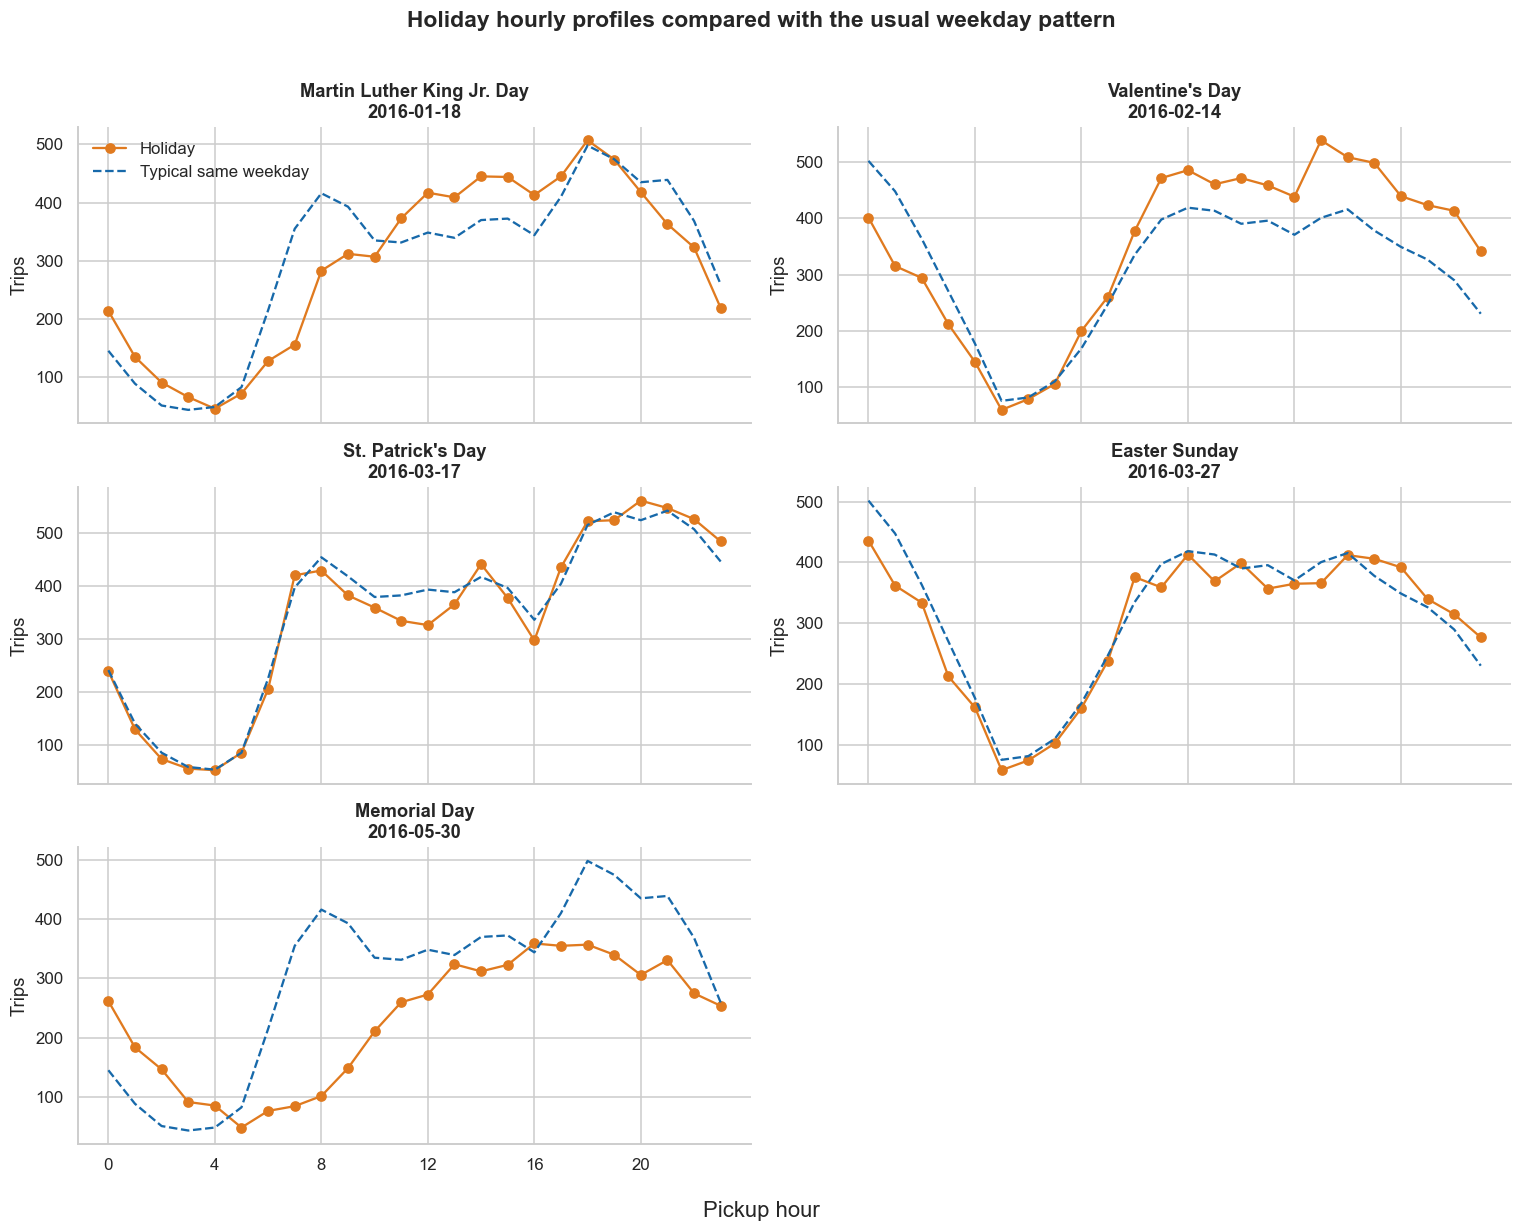
\includegraphics[width=0.95\linewidth]{figures/holiday_profiles.png}
  \caption{Hourly holiday profiles compared with the median profile of the
  same weekday. Holiday effects differ in both total volume and timing.}
  \label{fig:holidays}
\end{figure}

\subsection{Average speed throughout the day}

Figure~\ref{fig:speed} shows the mean and median trip speed by pickup hour.
Trips were fastest at 05:00, when the mean speed was 24.58 km/h and the median
was 22.84 km/h. Speed fell sharply from 06:00 as morning activity increased and
remained low through the working day. The lowest mean occurred at 15:00, at
12.14 km/h. Speed then increased after 19:00.

\begin{figure}[H]
  \centering
  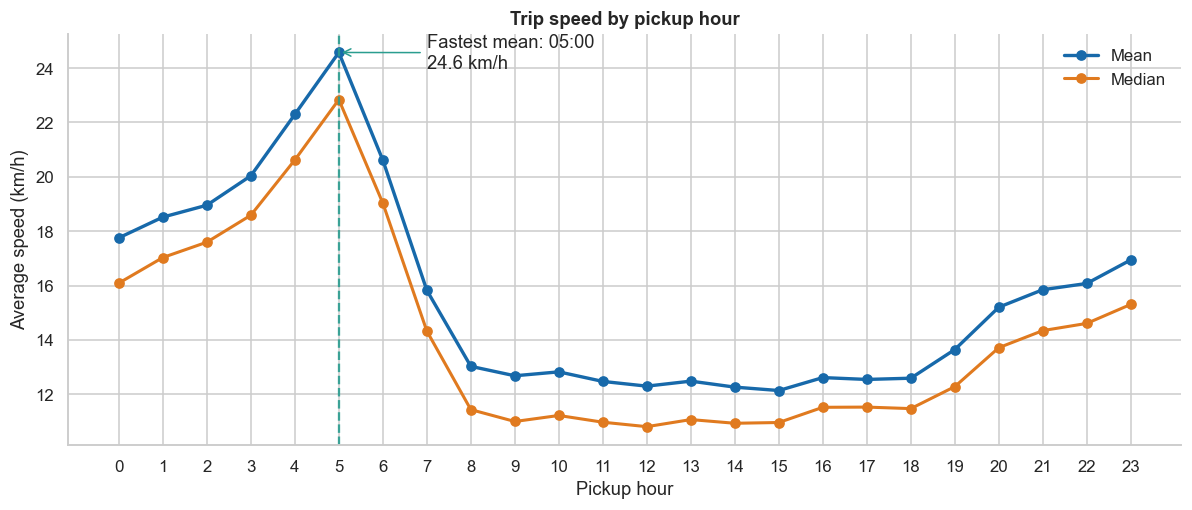
\includegraphics[width=0.9\linewidth]{figures/speed_by_hour.png}
  \caption{Mean and median average speed by pickup hour. Both measures show the
  same daily pattern.}
  \label{fig:speed}
\end{figure}

The agreement between the mean and median suggests that the pattern is not
caused only by a small number of unusually fast trips. Traffic congestion is
the most likely explanation, although route mix and trip distance may also
change during the day.

\section{Limitations}

The Haversine distance measures straight-line displacement and therefore
underestimates the road distance travelled. The training data are a sample of
recorded trips rather than a complete measure of taxi demand. The dataset also
does not contain journey purpose, traffic conditions or road routes. The
suggested explanations for commuting, nightlife and holiday activity are
therefore interpretations of the observed patterns, not causal conclusions.
Finally, each named holiday is represented by only one date in the six-month
period, so its result should not be generalised to every year.

\section{Conclusion}

The cleaning process removed 1.04\% of records and retained 1,443,535 plausible
trips. Friday had the highest average daily activity. Weekday demand was shaped
by commuting, while weekend demand shifted towards late-night travel. Memorial
Day showed the largest reduction relative to its normal weekday, whereas
Valentine's Day was busier than a typical Sunday. Trip speeds were highest in
the early morning and lowest during the congested daytime period. Together,
the results show that both trip volume and travel speed follow clear weekly and
hourly patterns.

\section*{Question 6: Dimensionality reduction}

\subsection{Sampled-trip feature matrix}

A random sample of exactly 20,000 cleaned trips is drawn without replacement
using seed 42. Each cleaned trip has the same chance of being selected. Original row indices and trip IDs are kept so each trip can be traced
back to the data, but IDs are not used as features. The full cleaned dataset
is still available for the time-based analysis.

The matrix contains 11 numeric features: pickup and drop-off longitude and
latitude (four columns), Haversine distance in kilometres, duration in minutes,
average speed in km/h, and two cyclic columns each for pickup hour and weekday.
Coordinates describe where trips start and end, and their direction.
Distance, duration and speed describe how far, how long and how fast trips
are. Hour and weekday capture daily and weekly travel patterns. Distance is
measured in a straight line, not along roads, so the speed estimate has the
same limitation. Speed is calculated from distance and duration. These three
features are therefore related and can give trip length and movement extra
weight in the analysis.

For pickup hour $h\in\{0,\ldots,23\}$, the encoding is
\begin{equation}
  h_{\sin}=\sin(2\pi h/24), \qquad h_{\cos}=\cos(2\pi h/24).
\end{equation}
Weekday uses the same encoding with a cycle of seven and Monday equal to zero.
This keeps midnight close to 23:00 and Monday close to Sunday, unlike using
the raw integers. Both sine and cosine are needed to tell positions around
the cycle apart. Raw hour and weekday are kept for interpretation but are
not added again to the matrix.

All 11 columns are standardized using \texttt{StandardScaler}, fitted on the
20,000 sampled rows:
\begin{equation}
  z_{ij}=\frac{x_{ij}-\mu_j}{\sigma_j},
  \qquad
  \sigma_j^2=\frac{1}{20000}\sum_{i=1}^{20000}(x_{ij}-\mu_j)^2.
\end{equation}
This gives each column a mean of zero and a population variance of one,
so different measurement units do not dominate distance-based methods.
Standardization does not remove skew or outliers; implausible extremes were
handled during cleaning. Scaling sine and cosine separately keeps the cycle
continuous but may stretch its circle into an ellipse. Each column has equal
variance, but groups of features do not necessarily have equal weight.
Distances between standardized coordinates are not exact geographic distances.

The notebook retains the encoded matrix as \texttt{X\_unscaled}, the
$20{,}000\times11$ standardized matrix as \texttt{X\_scaled}, and the fitted
scaler for reuse. Checks confirm the matrix shape, finite values, unique row
indices, matching row order, zero means and unit variances. These features
describe completed trips. Using duration or speed derived from duration to
predict duration would leak the target into the inputs. Any later train/test
analysis must fit its scaler on training rows only.

\subsection{Principal component analysis}

PCA was fitted using full singular value decomposition to the standardized
$20{,}000\times11$ feature matrix, without drawing a new sample. The scree plot
in Figure~\ref{fig:pca-scree} shows individual and cumulative explained
variance. PC1 explains 23.56\% and PC2 explains 14.11\%, giving
37.68\%. Eight components explain 89.63\%, below the required threshold;
\textbf{nine components are needed to explain at least 90\%}, retaining
94.58\%. The two-dimensional plot therefore leaves out most of the variance.

\begin{figure}[H]
  \centering
  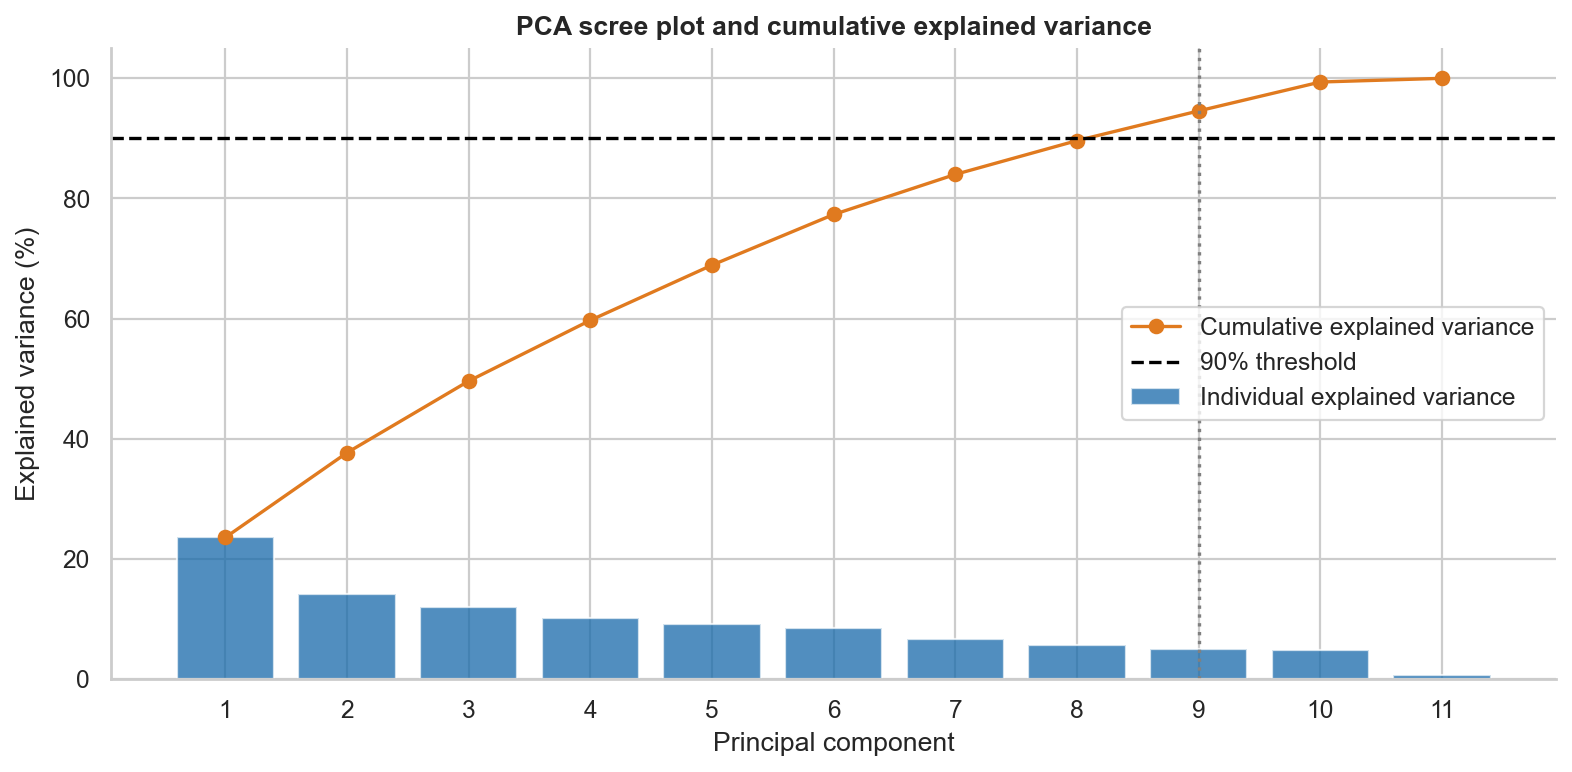
\includegraphics[width=\linewidth]{figures/pca_scree.png}
  \caption{Individual explained variance and its cumulative sum. The ninth
  component is the first to cross the 90\% threshold.}
  \label{fig:pca-scree}
\end{figure}

All 20,000 trips are shown on the first two components in
Figure~\ref{fig:pca-projections}, coloured by pickup hour, weekday/weekend and
Haversine distance. Colour values are matched to trips using the original
sampled row indices. Hour uses a cyclic colour map. Distance uses a logarithmic
colour scale to make the range easier to read; the PCA input is not log-transformed.
Distance increases clearly from left to right, including the extended
right-hand branch. Pickup-hour colours are mixed, while weekdays and
weekends overlap strongly in both the central cloud and the branch.
These plots do not prove that there are separate clusters, or that time
patterns are absent from the remaining components.

\begin{figure}[H]
  \centering
  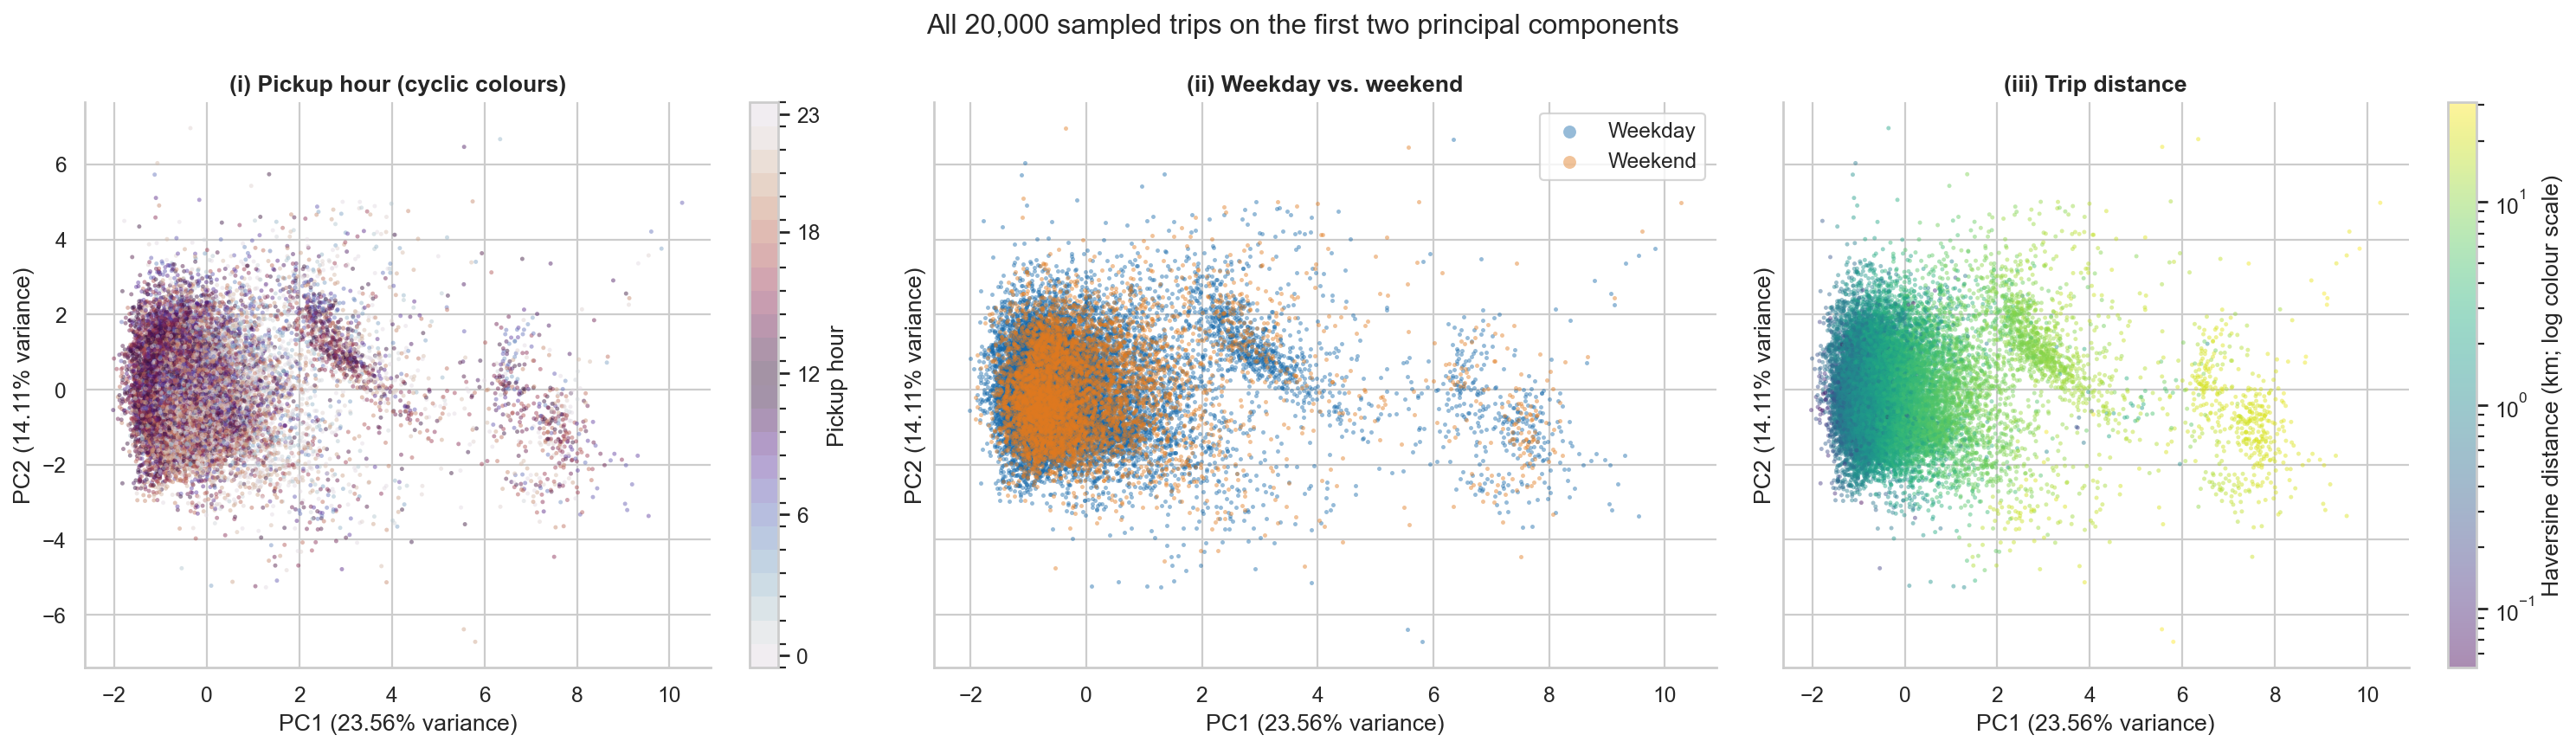
\includegraphics[width=\linewidth]{figures/pca_projections.png}
  \caption{PC1 and PC2 coloured by pickup hour (left), weekday/weekend (middle)
  and trip distance (right). The same trips and axes are used in each panel.}
  \label{fig:pca-projections}
\end{figure}

Figure~\ref{fig:pca-loadings} gives the signed component coefficients, here
called loadings. They are the weights used to combine the centered,
standardized features, not correlations between features and component scores.
Reversing all signs in a component does not change the PCA solution.

\begin{figure}[H]
  \centering
  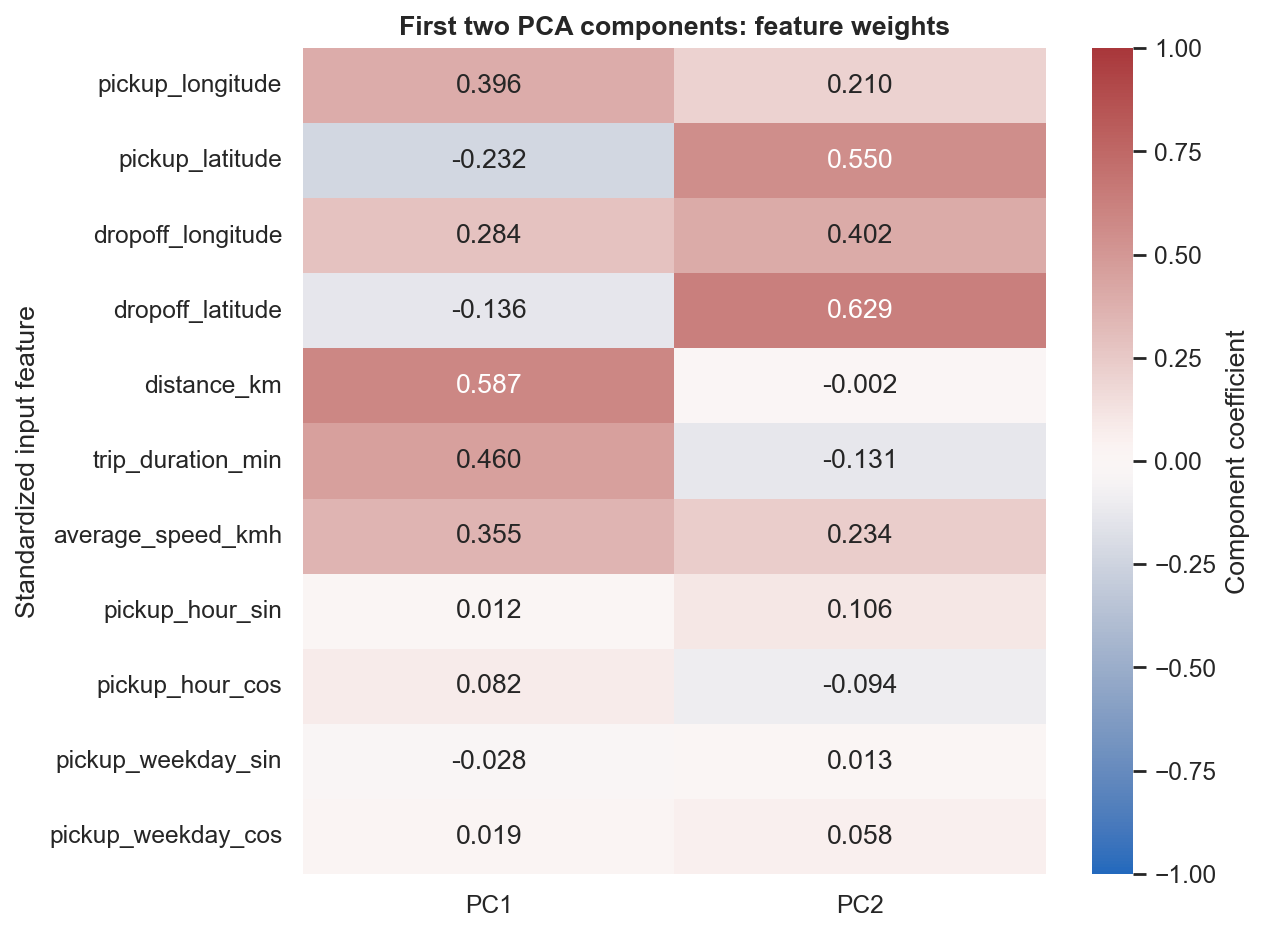
\includegraphics[width=0.8\linewidth]{figures/pca_loadings.png}
  \caption{Feature coefficients of the first two principal components.}
  \label{fig:pca-loadings}
\end{figure}

\textbf{PC1 mainly represents trip length, duration and speed, with a location effect.}
The strongest coefficients are distance ($+0.588$), duration ($+0.459$),
pickup longitude ($+0.396$), speed ($+0.355$) and drop-off longitude ($+0.284$).
Higher scores tend to describe longer-distance, longer-duration and faster
trips, with pickup and drop-off points farther east. Negative latitude weights
also link higher scores to points farther south. This is not a distance-only
axis. Because speed depends on distance and duration, these related features
have a combined influence.

\textbf{PC2 is primarily a north-east versus south-west location axis.}
Drop-off latitude ($+0.629$), pickup latitude ($+0.550$), drop-off longitude
($+0.402$) and pickup longitude ($+0.210$) have the largest weights. Higher
scores generally indicate pickup and drop-off points farther north and east.
Speed ($+0.234$) and duration ($-0.131$) also link higher scores to faster,
shorter-duration trips, while distance
has almost no direct weight ($-0.0015$). Hour and weekday coefficients are
small on both components, matching the mixed time-based colours. These
describe linear relationships, not causes or confirmed reasons for travel.

\subsection{t-SNE and perplexity}

Three two-dimensional t-SNE embeddings were fitted to the same standardized
$20{,}000\times11$ matrix, at perplexities 5, 30 and 100. No further sampling or
reduction to two PCA components was used. All other settings were fixed:
Euclidean distance, PCA initialization, seed 42, automatic learning rate
(416.67 for this sample), early exaggeration 12, 1,000 maximum iterations,
and Barnes--Hut approximation with angle 0.5. Computation was limited to two
threads. All runs used the full iteration budget. This does not show that
they converged or that results are stable across different seeds.

Perplexity controls how many nearby points influence the input similarities,
not the number of clusters. Figure~\ref{fig:tsne} compares the
embeddings using the same hour and distance colour scales. Each row repeats
one embedding, coloured by pickup hour, weekday/weekend and distance.
The distance colour scale is logarithmic for readability; the input distance
feature was standardized without a log transform.

\begin{figure}[H]
  \centering
  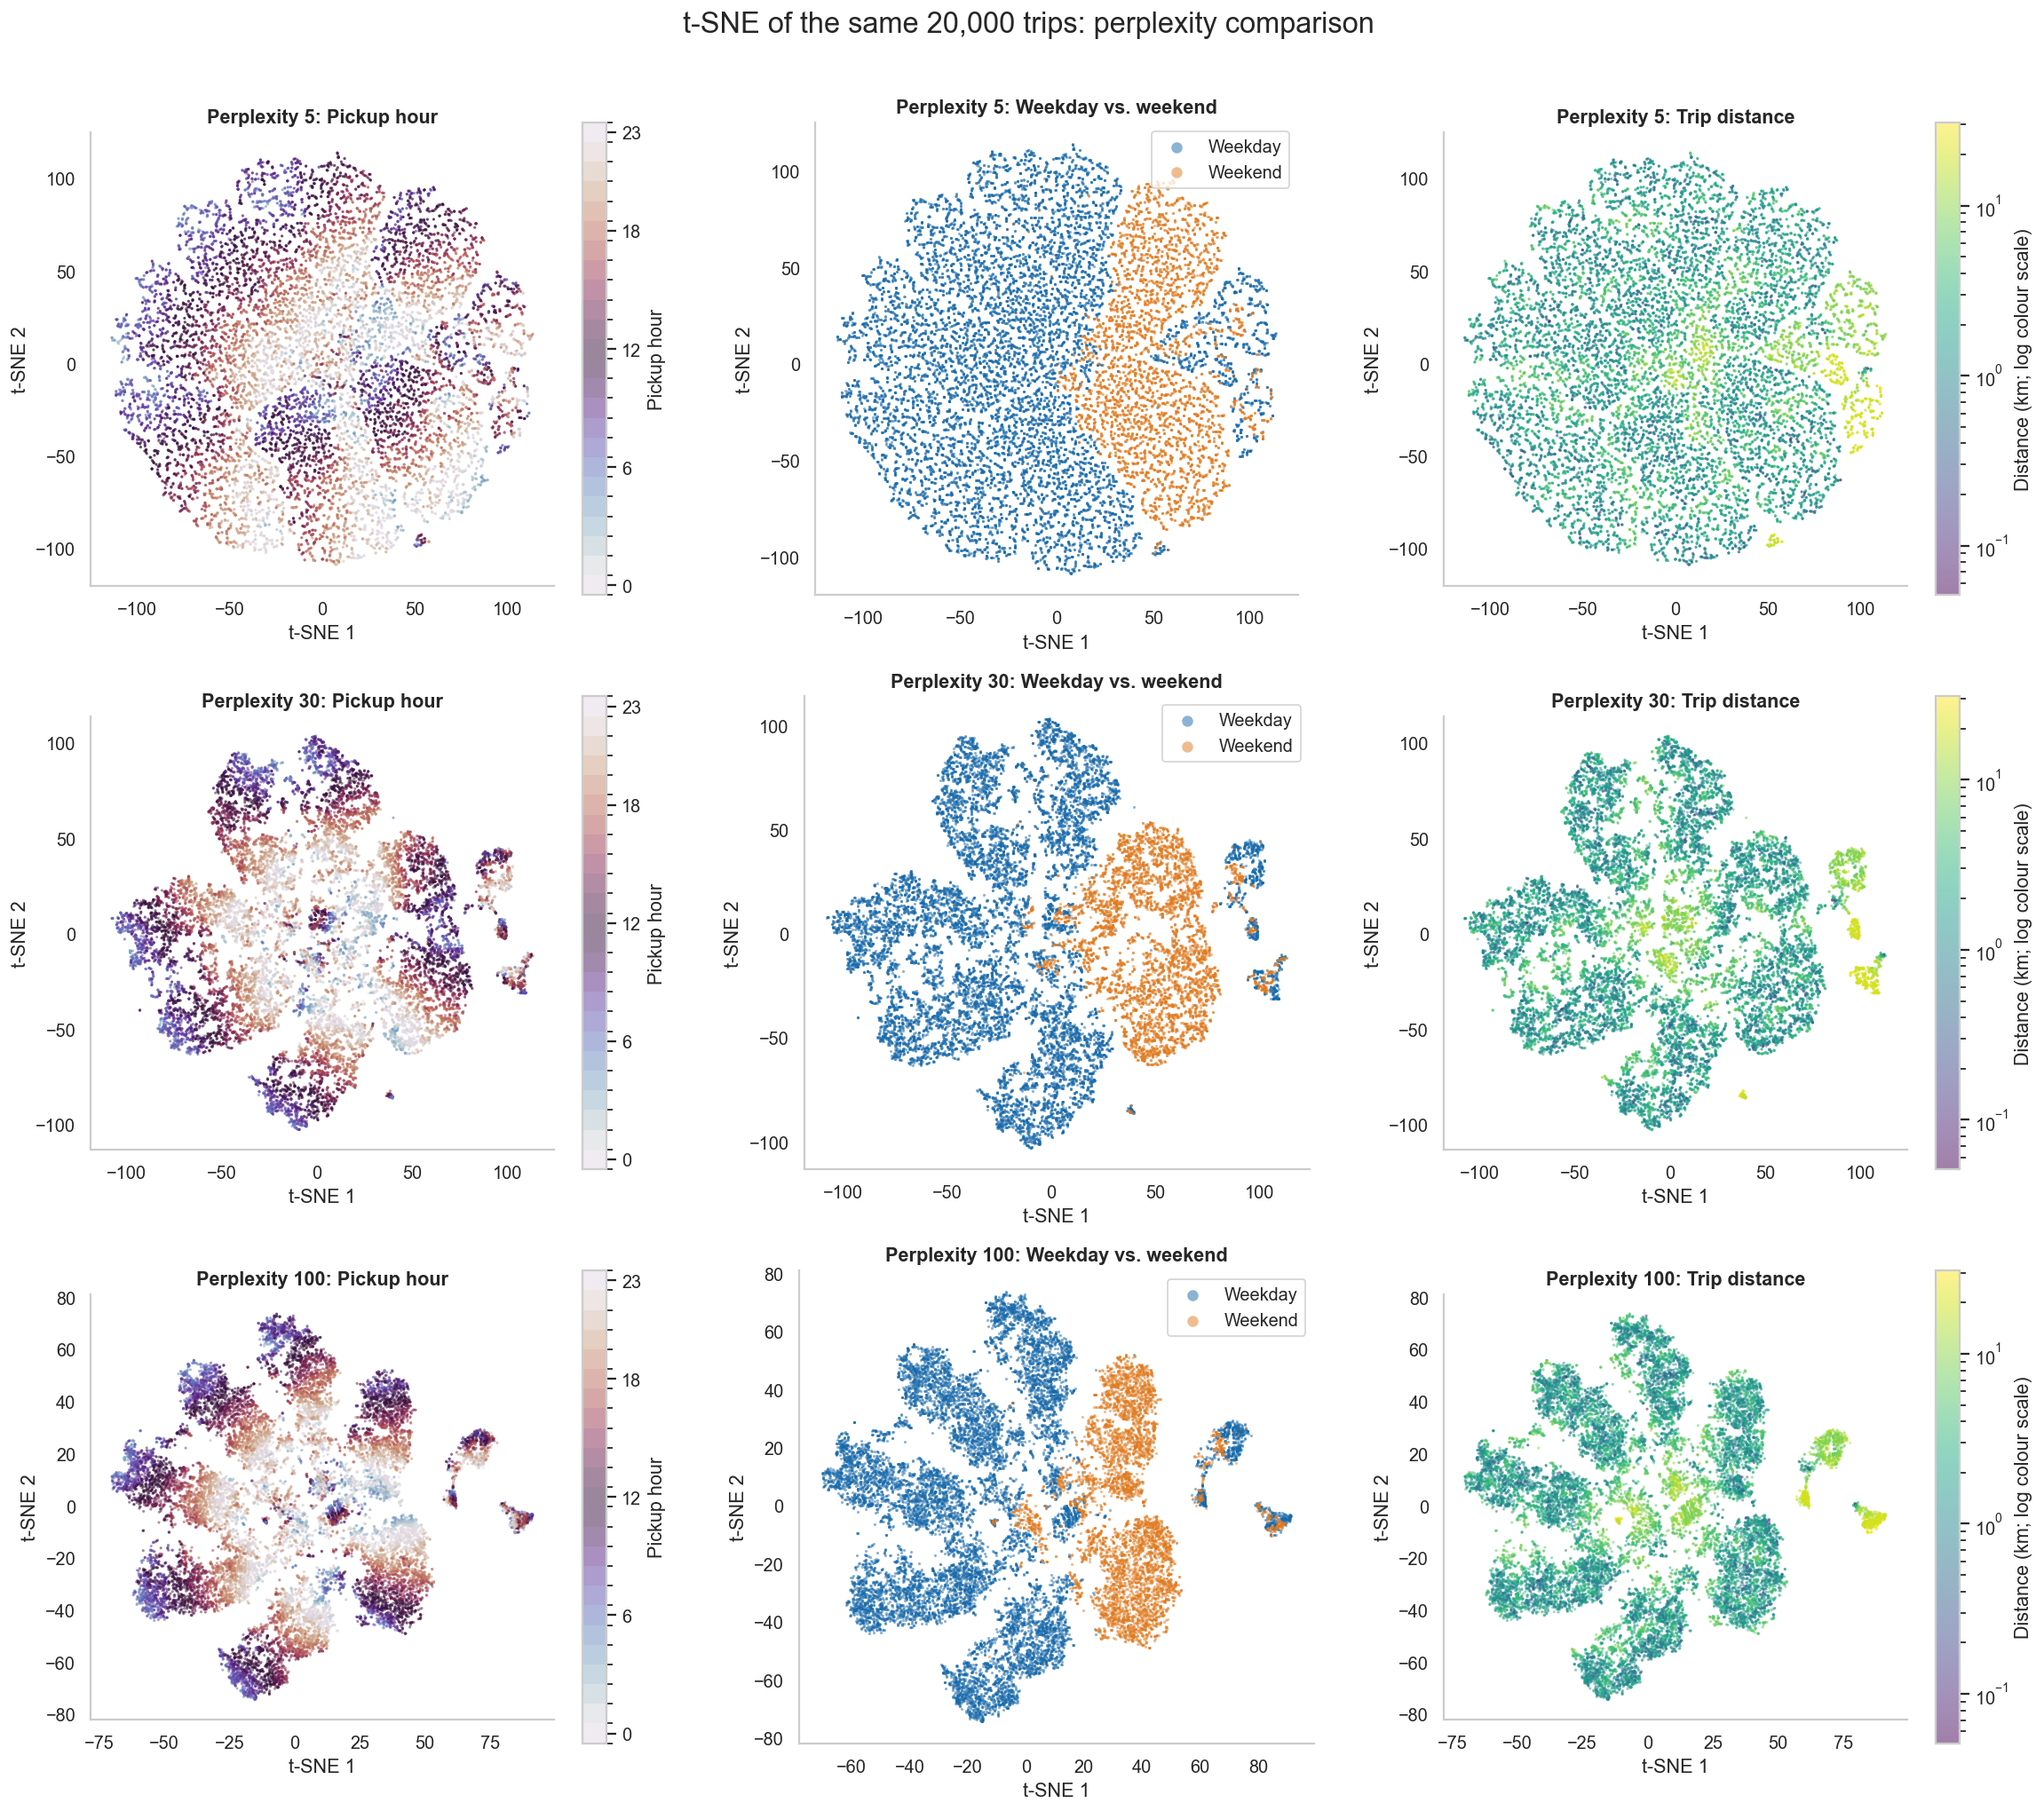
\includegraphics[width=\linewidth]{figures/tsne_perplexity_comparison.png}
  \caption{t-SNE for perplexities 5, 30 and 100 (rows), coloured by pickup hour,
  weekday/weekend and Haversine distance (columns). All 20,000 trips appear
  in every panel.}
  \label{fig:tsne}
\end{figure}

\textbf{Perplexity 5} produces a roughly disk-shaped map with thin strands
and small patches, with fewer clear gaps between broad regions. Hour varies
locally and weekend trips concentrate in a right-hand region, but the fine
texture makes broad neighbourhoods harder to read.

\textbf{Perplexity 30} produces clearer lobes and gaps, with nearby points
showing similar hour colours. Weekend trips occupy clear right-hand lobes,
whereas weekday trips dominate the left and upper/lower regions. Longer
trips concentrate in a small separated right-hand branch, although distance
also varies within the main map.

\textbf{Perplexity 100} keeps broadly similar colour patterns and
the long-distance side branch, while producing more compact lobes with less
fine strand-like detail. Larger perplexity therefore changes the level of detail
and layout; in these data it makes broad lobes clearer rather than simply
merging everything into one cloud. Perplexity 30 offers a useful middle-scale
view, but these plots do not prove that it is the best setting.

Interpret nearby relationships with care. t-SNE axes have no feature
loadings or explained-variance meaning, and the ordering, areas and distances
between separate islands do not reliably describe the original feature space.
An island is not proof of a real cluster. Hour, weekday and distance are
already input features, so similar colours do not independently confirm trip
classes. Final KL divergence shows how well each run fits its target
similarities. It cannot be used directly to choose between perplexities,
because each perplexity changes those target similarities.

\subsection{UMAP: neighbourhood size and minimum distance}

UMAP was fitted to the same standardized $20{,}000\times11$ matrix for all
six combinations of \texttt{n\_neighbors} equal to 5, 15 and 50 and
\texttt{min\_dist} equal to 0.0 and 0.5. No additional sampling or
reduction to two PCA components was used. Euclidean distance, spectral
initialization, spread 1.0, 500 optimization epochs and seed 42 were fixed.
Seeded optimization used one worker; numerical thread pools were limited to
two threads. The implementation uses the \texttt{umap-learn} package.

\texttt{n\_neighbors} controls the graph linking nearby input points:
small values focus on very local structure, while larger values include
broader connections. \texttt{min\_dist} controls how tightly points can
pack in the plot. It is not a strict minimum distance or a threshold on
distances in the input data. Figures~\ref{fig:umap-zero} and~\ref{fig:umap-half}
hold minimum distance fixed and vary neighbourhood size by row. All panels
use the same colour scales and all 20,000 trips, with labels added after
fitting. Distance uses a log colour scale only.

\begin{figure}[H]
  \centering
  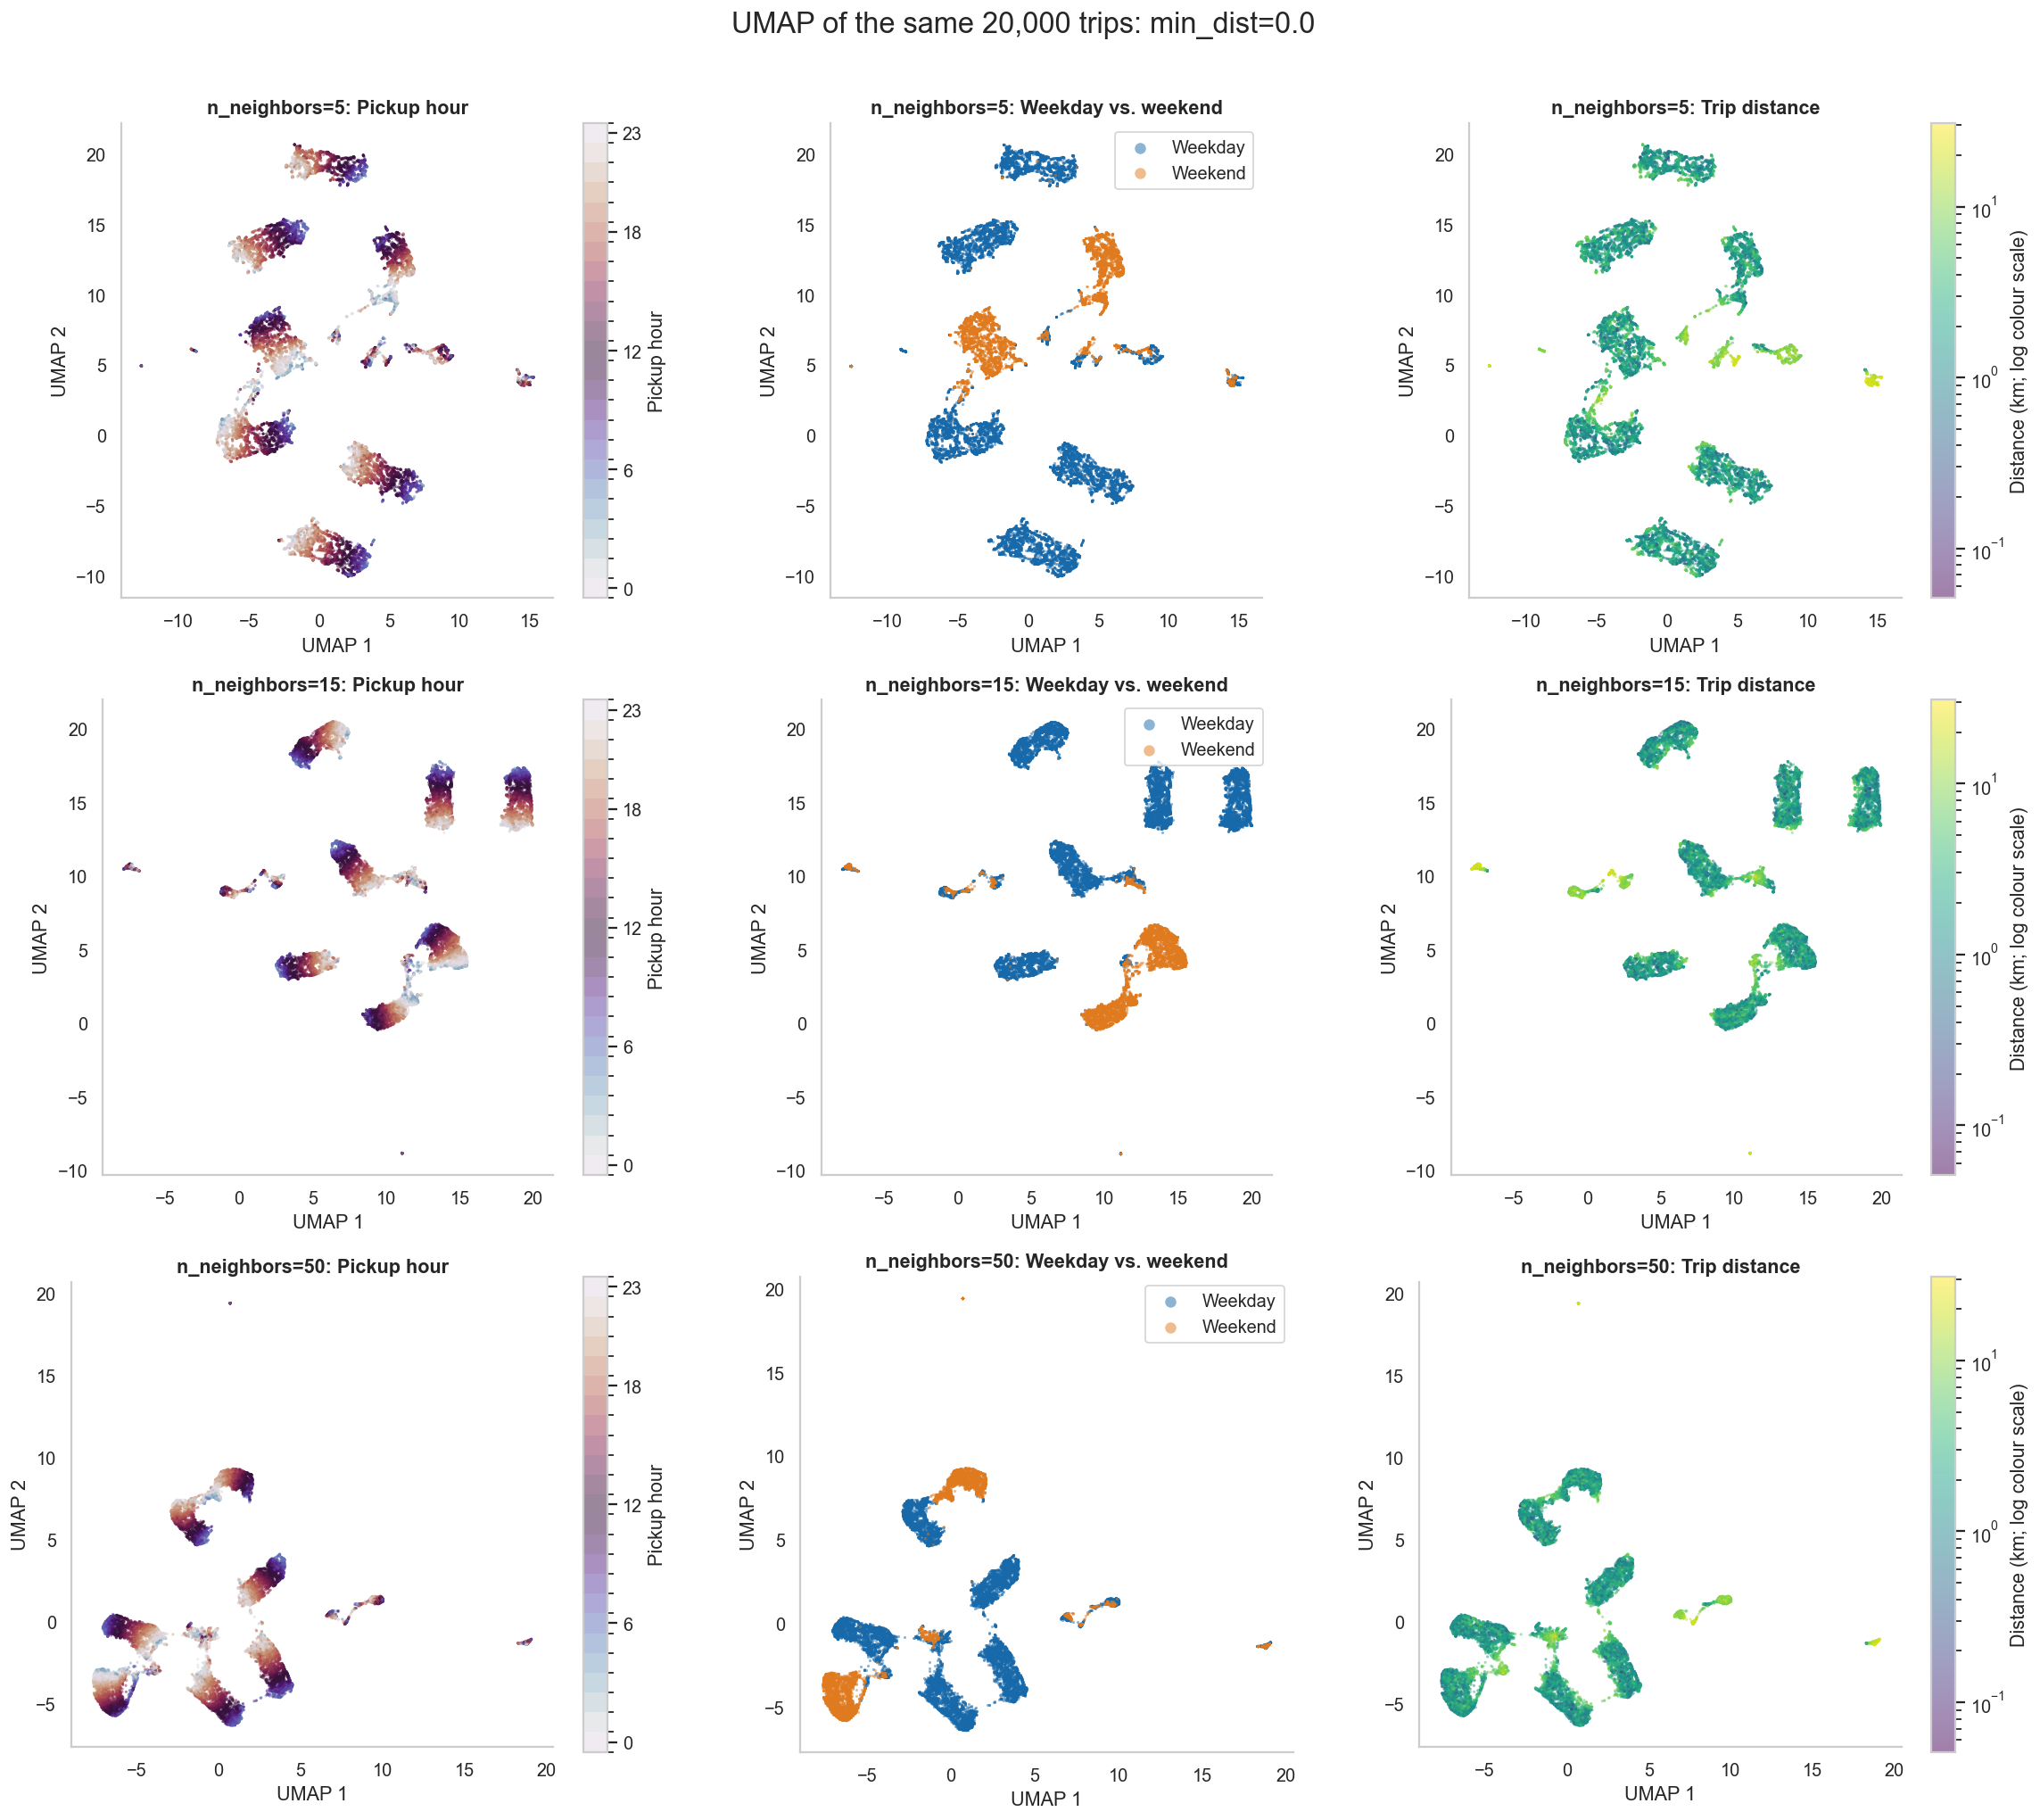
\includegraphics[width=\linewidth]{figures/umap_min_dist_0.0.png}
  \caption{UMAP with minimum distance 0.0. Rows use 5, 15 and 50 neighbours;
  columns show pickup hour, weekday/weekend and Haversine distance.}
  \label{fig:umap-zero}
\end{figure}

\begin{figure}[H]
  \centering
  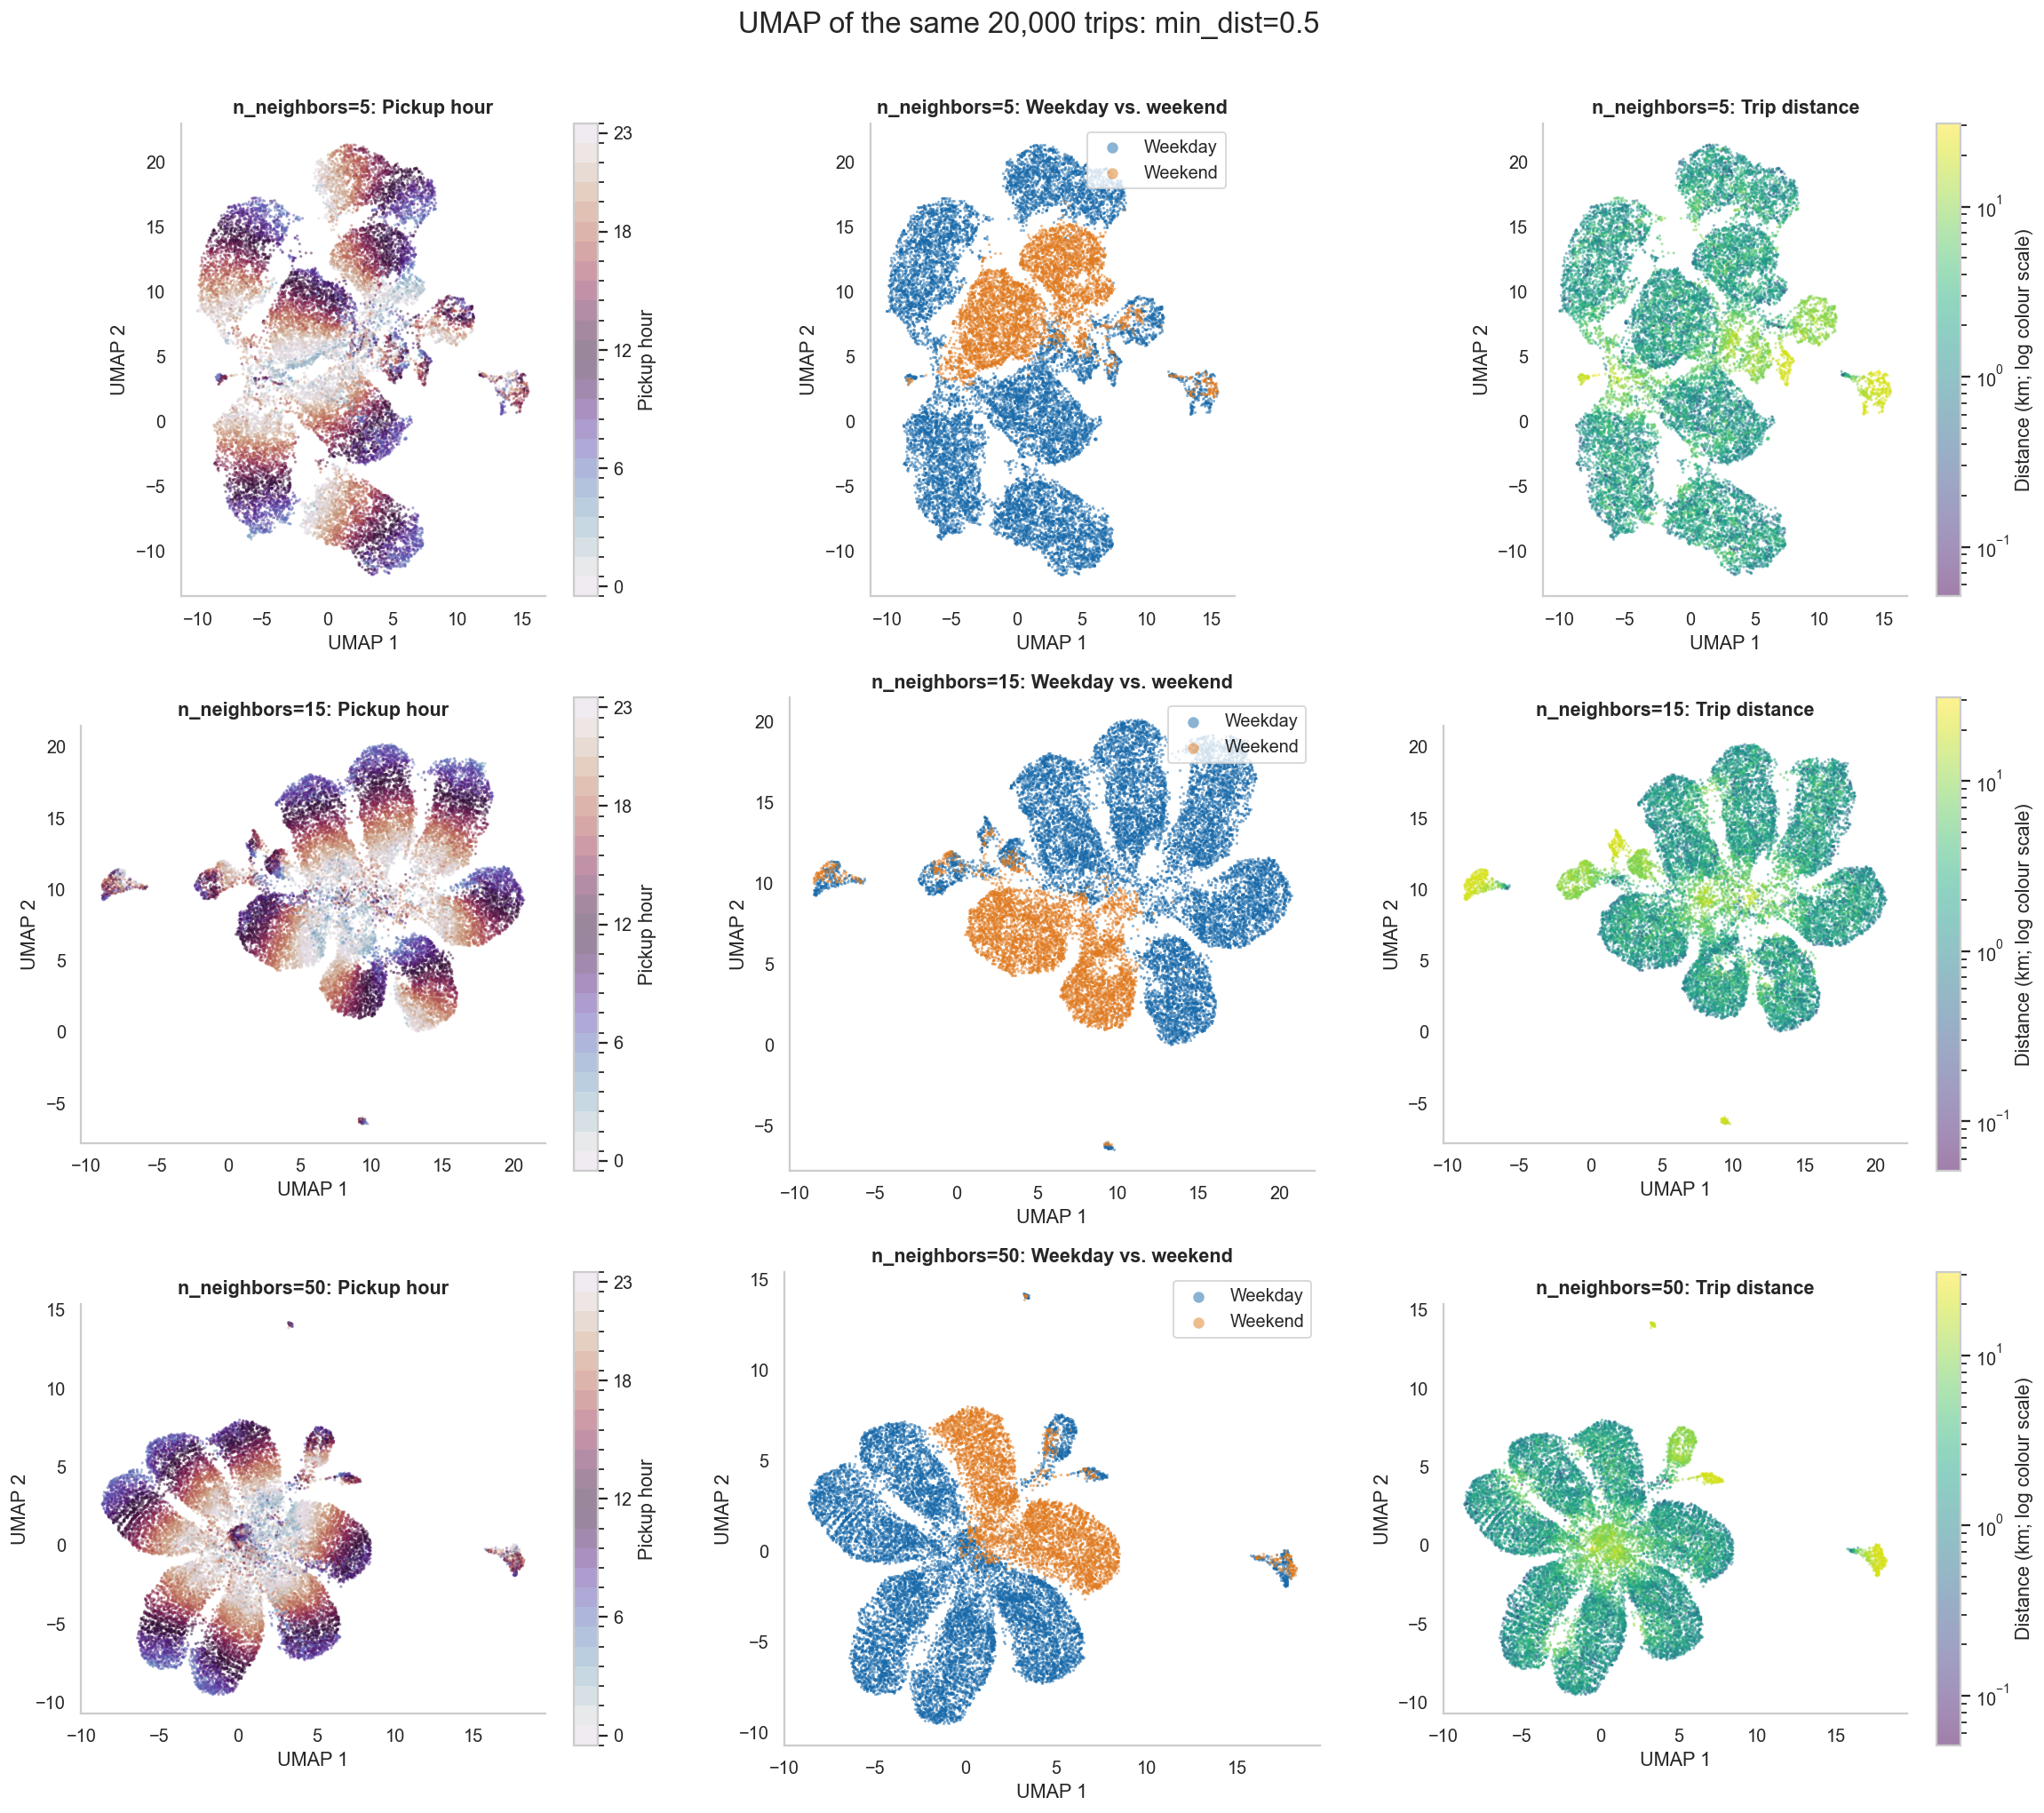
\includegraphics[width=\linewidth]{figures/umap_min_dist_0.5.png}
  \caption{UMAP with minimum distance 0.5, using the same row and colour
  conventions as Figure~\ref{fig:umap-zero}.}
  \label{fig:umap-half}
\end{figure}

\textbf{Effect of neighbourhood size.} With 5 neighbours, several compact
islands and small outlying groups are visible at minimum distance 0.0; at 0.5
the islands expand into broader lobes but remain partly separated.
With 15 neighbours, the 0.0 map still has separate islands, whereas
the 0.5 map connects main lobes around a central region, with readable
hour changes within each lobe. With 50 neighbours, broader connections
reduce some separation: at 0.0 some lobes join but islands remain,
while at 0.5 the main body is much more connected. Small long-distance
outlying groups remain. Increasing neighbourhood size therefore does not
simply force all observations into one group.

\textbf{Effect of minimum distance.} Holding neighbourhood size fixed,
0.0 allows tight packing and yields compact, sharply separated islands.
At 0.5, lobes occupy more area, gaps narrow and bridges become more visible,
particularly with 15 or 50 neighbours. This changes visual compactness
rather than the number of input neighbours.

\textbf{Colour patterns and interpretation.} Gradual changes in pickup hour
and regions dominated by weekdays or weekends appear in all six runs.
Longer trips concentrate in small branches, outlying groups and areas
near the main body. Distance is more mixed within the large time-based lobes.
Changing parameters moves and reshapes these regions. Since time and distance
are input features, their colours do not independently confirm trip classes.
Fifteen neighbours with minimum distance 0.5 gives a useful middle-scale
view, but appearance alone does not prove that it is the best setting.
The axes have no loadings or explained-variance meaning. Island spacing,
area and apparent density do not exactly represent the original feature
space. Islands are not proof of real clusters or reasons for travel.
A fixed seed and 500 epochs do not show convergence or stability across
seeds or library versions.

\subsection{Density-based clustering in the reduced spaces}

HDBSCAN from \texttt{sklearn.cluster} was fitted in three spaces: all nine
PCA components needed to explain at least 90\% variance, the selected
perplexity-30 t-SNE embedding, and UMAP with 15 neighbours and minimum
distance 0.5. The t-SNE and UMAP settings were chosen for readable
middle-scale views, not to obtain particular cluster counts. Reduced
coordinates were not whitened or rescaled separately. PCA labels are shown on PC1
and PC2 only, although clustering uses nine dimensions.

The minimum cluster size was 200 (1\% of the sample), so tiny groups were
not treated as main trip classes. The density requirement was
\texttt{min\_samples=20}, just above twice the largest dimension, nine.
Euclidean distance, excess-of-mass hierarchy selection, no additional
epsilon merging, and \texttt{allow\_single\_cluster=False} were used.
Unlike DBSCAN, HDBSCAN selects groups that persist across a hierarchy of
distance scales, so it does not need one epsilon or a k-distance elbow.
These settings help explore the data; they do not estimate the true trip classes.

\begin{table}[H]
  \caption{HDBSCAN results for the same 20,000 sampled trips. Noise is excluded
  from the cluster count.}
  \centering
  \begin{tabular}{lrrrr}
    \toprule
    Space & Dimensions & Clusters & Noise trips & Noise (\%) \\
    \midrule
    PCA & 9 & 3 & 1,736 & 8.680 \\
    t-SNE & 2 & 3 & 57 & 0.285 \\
    UMAP & 2 & 2 & 53 & 0.265 \\
    \bottomrule
  \end{tabular}
\end{table}

\begin{figure}[H]
  \centering
  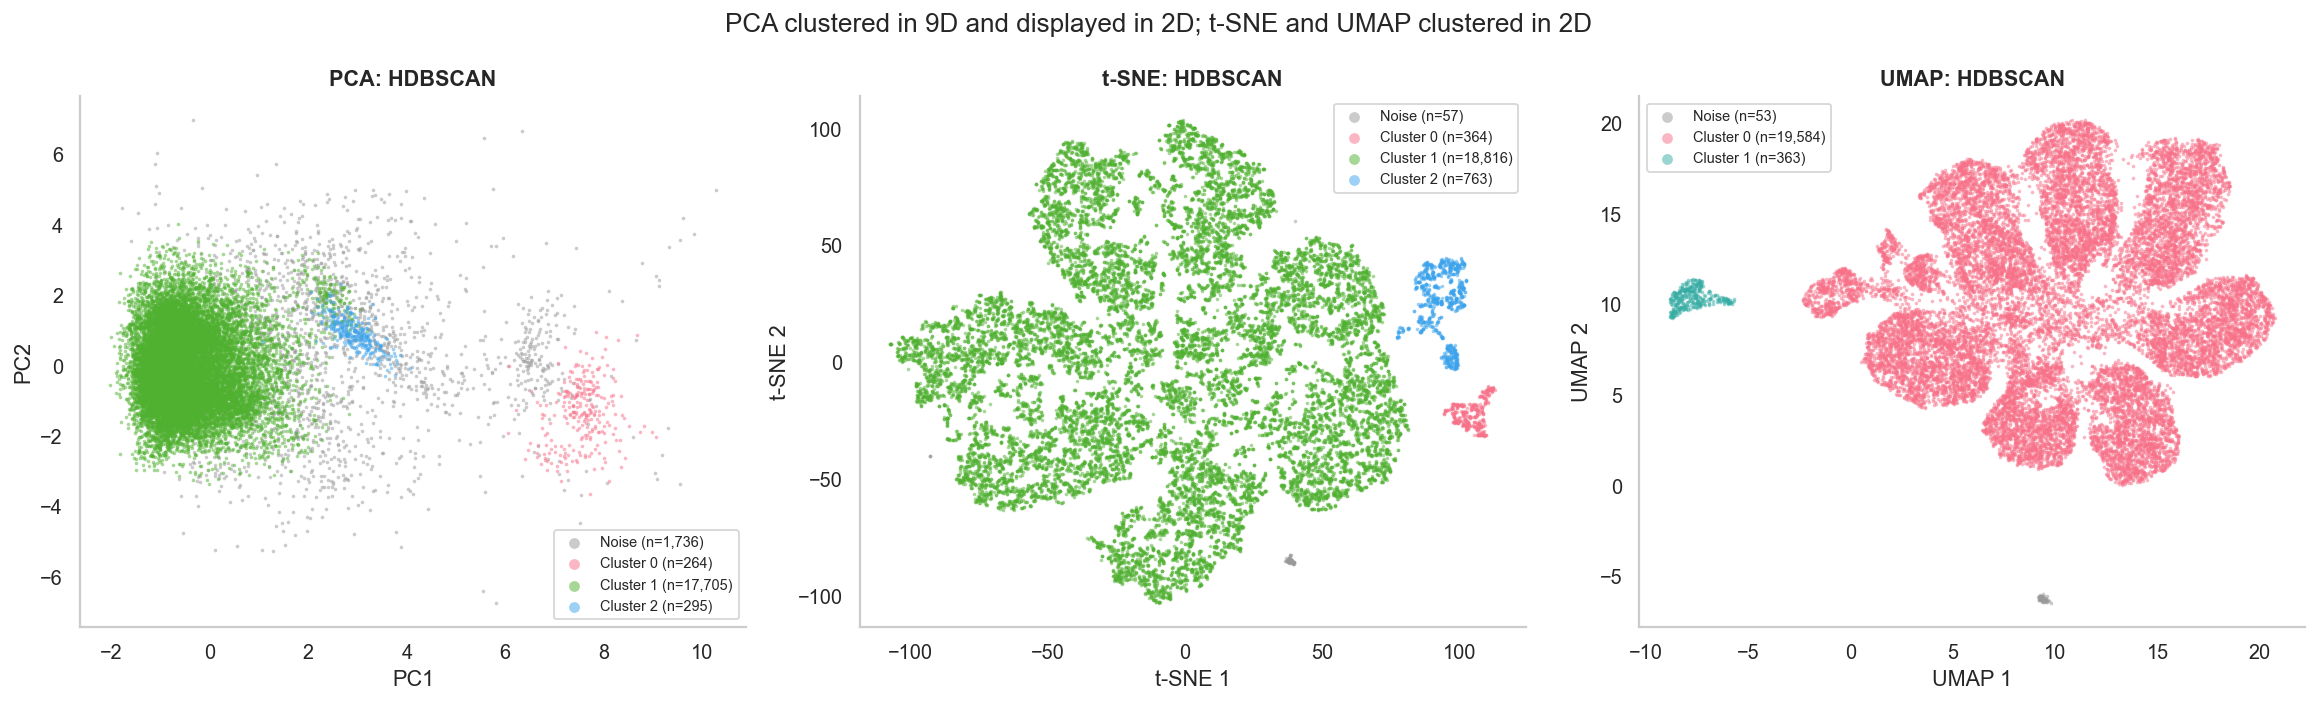
\includegraphics[width=\linewidth]{figures/clustering_projections.png}
  \caption{HDBSCAN labels in the three reduced spaces. PCA is clustered in
  nine dimensions and displayed on the first two. Grey points are noise;
  cluster numbers apply only within each space.}
  \label{fig:cluster-projections}
\end{figure}

\subsubsection{Parameter sensitivity}

Minimum cluster sizes 100, 200 and 400 were compared at
\texttt{min\_samples=20}; density settings 10, 20 and 40 were compared at
cluster size 200. The notebook also reports adjusted Rand indices against
the chosen clustering, including noise. At cluster size 200, PCA gives
9, 3 and 2 clusters for density settings 10, 20 and 40, with noise
23.445\%, 8.680\% and 1.910\%. The PCA clustering is therefore not stable
across these settings. t-SNE keeps three clusters across these
density settings (0.285--0.515\% noise), and UMAP retains two (0.265\% noise).
At cluster size 400, the smaller JFK groups are too small to be selected:
PCA produces seven clusters and 36.810\% noise, t-SNE produces two and
2.105\% noise, and UMAP produces eight and 11.470\% noise.
Changing which groups meet the size limit can change the selected hierarchy.
Cluster counts and noise therefore need not always rise or fall together.
A high adjusted Rand index may mainly reflect the large shared urban group,
rather than stable small airport groups.

\begin{figure}[H]
  \centering
  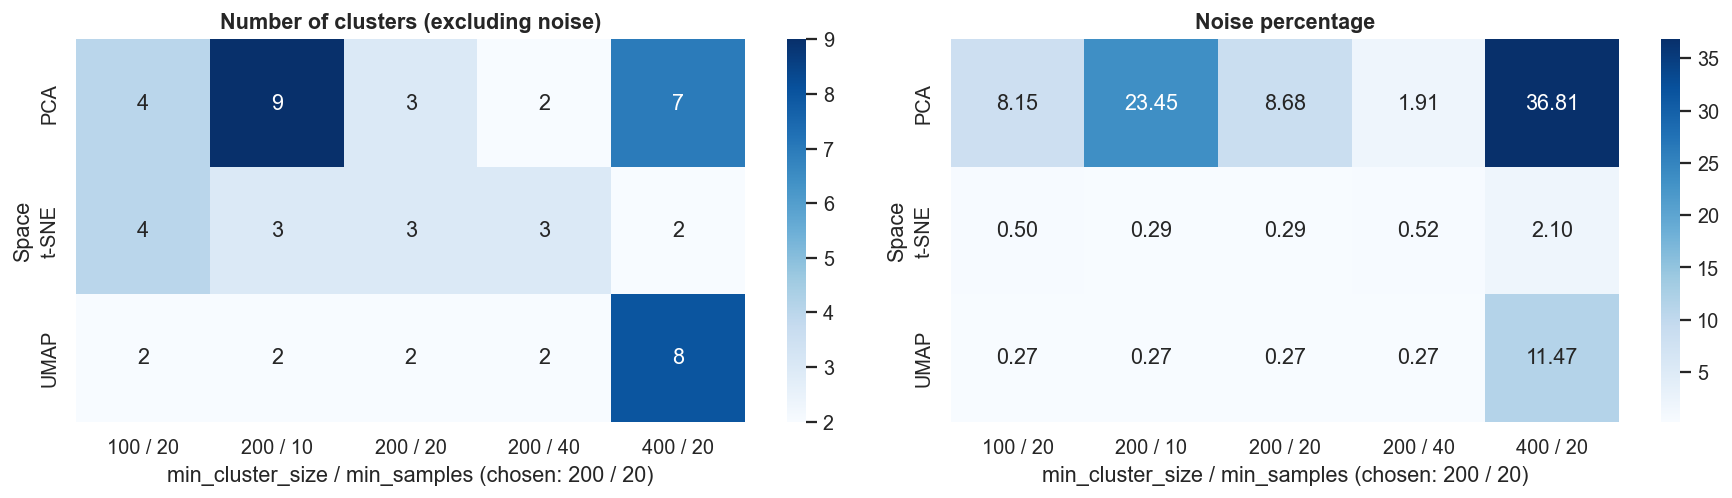
\includegraphics[width=\linewidth]{figures/clustering_sensitivity.png}
  \caption{Cluster counts and noise percentages for five parameter settings.
  The selected setting is minimum cluster size 200 and minimum samples 20.}
  \label{fig:cluster-sensitivity}
\end{figure}

\subsubsection{Original-feature profiles and descriptive names}

Profiles use unscaled trip records, with duration in minutes, Haversine
distance in kilometres and implied speed in km/h. Both the median and most
frequent (modal) hour are reported because a linear hour median can mislead across
midnight. Short means median distance below 3 km, medium-distance means
3 to below 12 km, and long-distance means at least 12 km. Weekday-heavy
means at least 65\% weekdays. It does not mean more weekdays than expected
from the sample, which already contains more weekdays. No six-hour time band contains half of
any selected cluster, so all are described as mixed-hour.

\begin{table}[H]
  \caption{Original-unit profiles for every cluster and noise group (-1).
  Hours are median/mode; Wd and We denote weekday and weekend percentages.}
  \centering
  \resizebox{\linewidth}{!}{%
  \begin{tabular}{llrrrrrrr}
    \toprule
    Space & Label & Trips & Distance & Duration & Speed & Hours & Wd (\%) & We (\%) \\
    \midrule
    PCA & -1 & 1,736 & 9.13 & 24.29 & 23.09 & 13/22 & 70.45 & 29.55 \\
    PCA & 0 & 264 & 20.15 & 44.27 & 26.08 & 16/14 & 65.15 & 34.85 \\
    PCA & 1 & 17,705 & 1.88 & 10.05 & 12.14 & 14/18 & 71.92 & 28.08 \\
    PCA & 2 & 295 & 9.74 & 31.35 & 18.61 & 16/22 & 82.71 & 17.29 \\
    \midrule
    t-SNE & -1 & 57 & 17.88 & 37.93 & 28.97 & 13/14 & 78.95 & 21.05 \\
    t-SNE & 0 & 364 & 19.80 & 38.91 & 26.03 & 15/14 & 65.93 & 34.07 \\
    t-SNE & 1 & 18,816 & 1.96 & 10.42 & 12.42 & 14/18 & 71.72 & 28.28 \\
    t-SNE & 2 & 763 & 10.16 & 29.67 & 21.38 & 15/22 & 77.72 & 22.28 \\
    \midrule
    UMAP & -1 & 53 & 18.03 & 38.23 & 29.29 & 13/14 & 77.36 & 22.64 \\
    UMAP & 0 & 19,584 & 2.04 & 10.74 & 12.67 & 14/18 & 71.96 & 28.04 \\
    UMAP & 1 & 363 & 19.80 & 38.93 & 26.07 & 15/14 & 65.84 & 34.16 \\
    \bottomrule
  \end{tabular}%
  }
\end{table}

The names and geographic evidence are as follows; all named groups are
weekday-heavy and mixed-hour.
\begin{itemize}
  \item \textbf{PCA 0: long-distance JFK-area pickups.}
  98.11\% of pickups are within 2 km of the approximate JFK reference point.
  \item \textbf{PCA 1: short urban trips.}
  The pickup map is concentrated in the Manhattan corridor.
  \item \textbf{PCA 2: medium-distance LaGuardia-area pickups.}
  99.32\% are within 2 km of the LaGuardia reference point.
  \item \textbf{t-SNE 0: long-distance JFK-area pickups.}
  96.15\% are near JFK.
  \item \textbf{t-SNE 1: short urban trips.}
  This broad group covers the main urban pickup corridor.
  \item \textbf{t-SNE 2: medium-distance LaGuardia-area pickups.}
  74.44\% are near LaGuardia; pickups are more spread out than in PCA cluster 2.
  \item \textbf{UMAP 0: short urban trips.}
  This broad group also absorbs LaGuardia-area trips.
  \item \textbf{UMAP 1: long-distance JFK-area pickups.}
  96.42\% are near JFK.
\end{itemize}

Airport proximity is measured using Haversine distance to approximate
reference points. An airport-area name requires at least 50\% of pickups
within 2 km. This does not prove terminal use or the reason for travel.
Figures~\ref{fig:cluster-pca-map}--\ref{fig:cluster-umap-map} plot every
cluster's pickup locations separately, including noise for comparison.
These are offline longitude/latitude maps with the same geographic limits
and an aspect ratio adjusted for local latitude, not street or route maps. Reference landmarks
provide context and grey background points show all sampled pickups.

\begin{figure}[H]
  \centering
  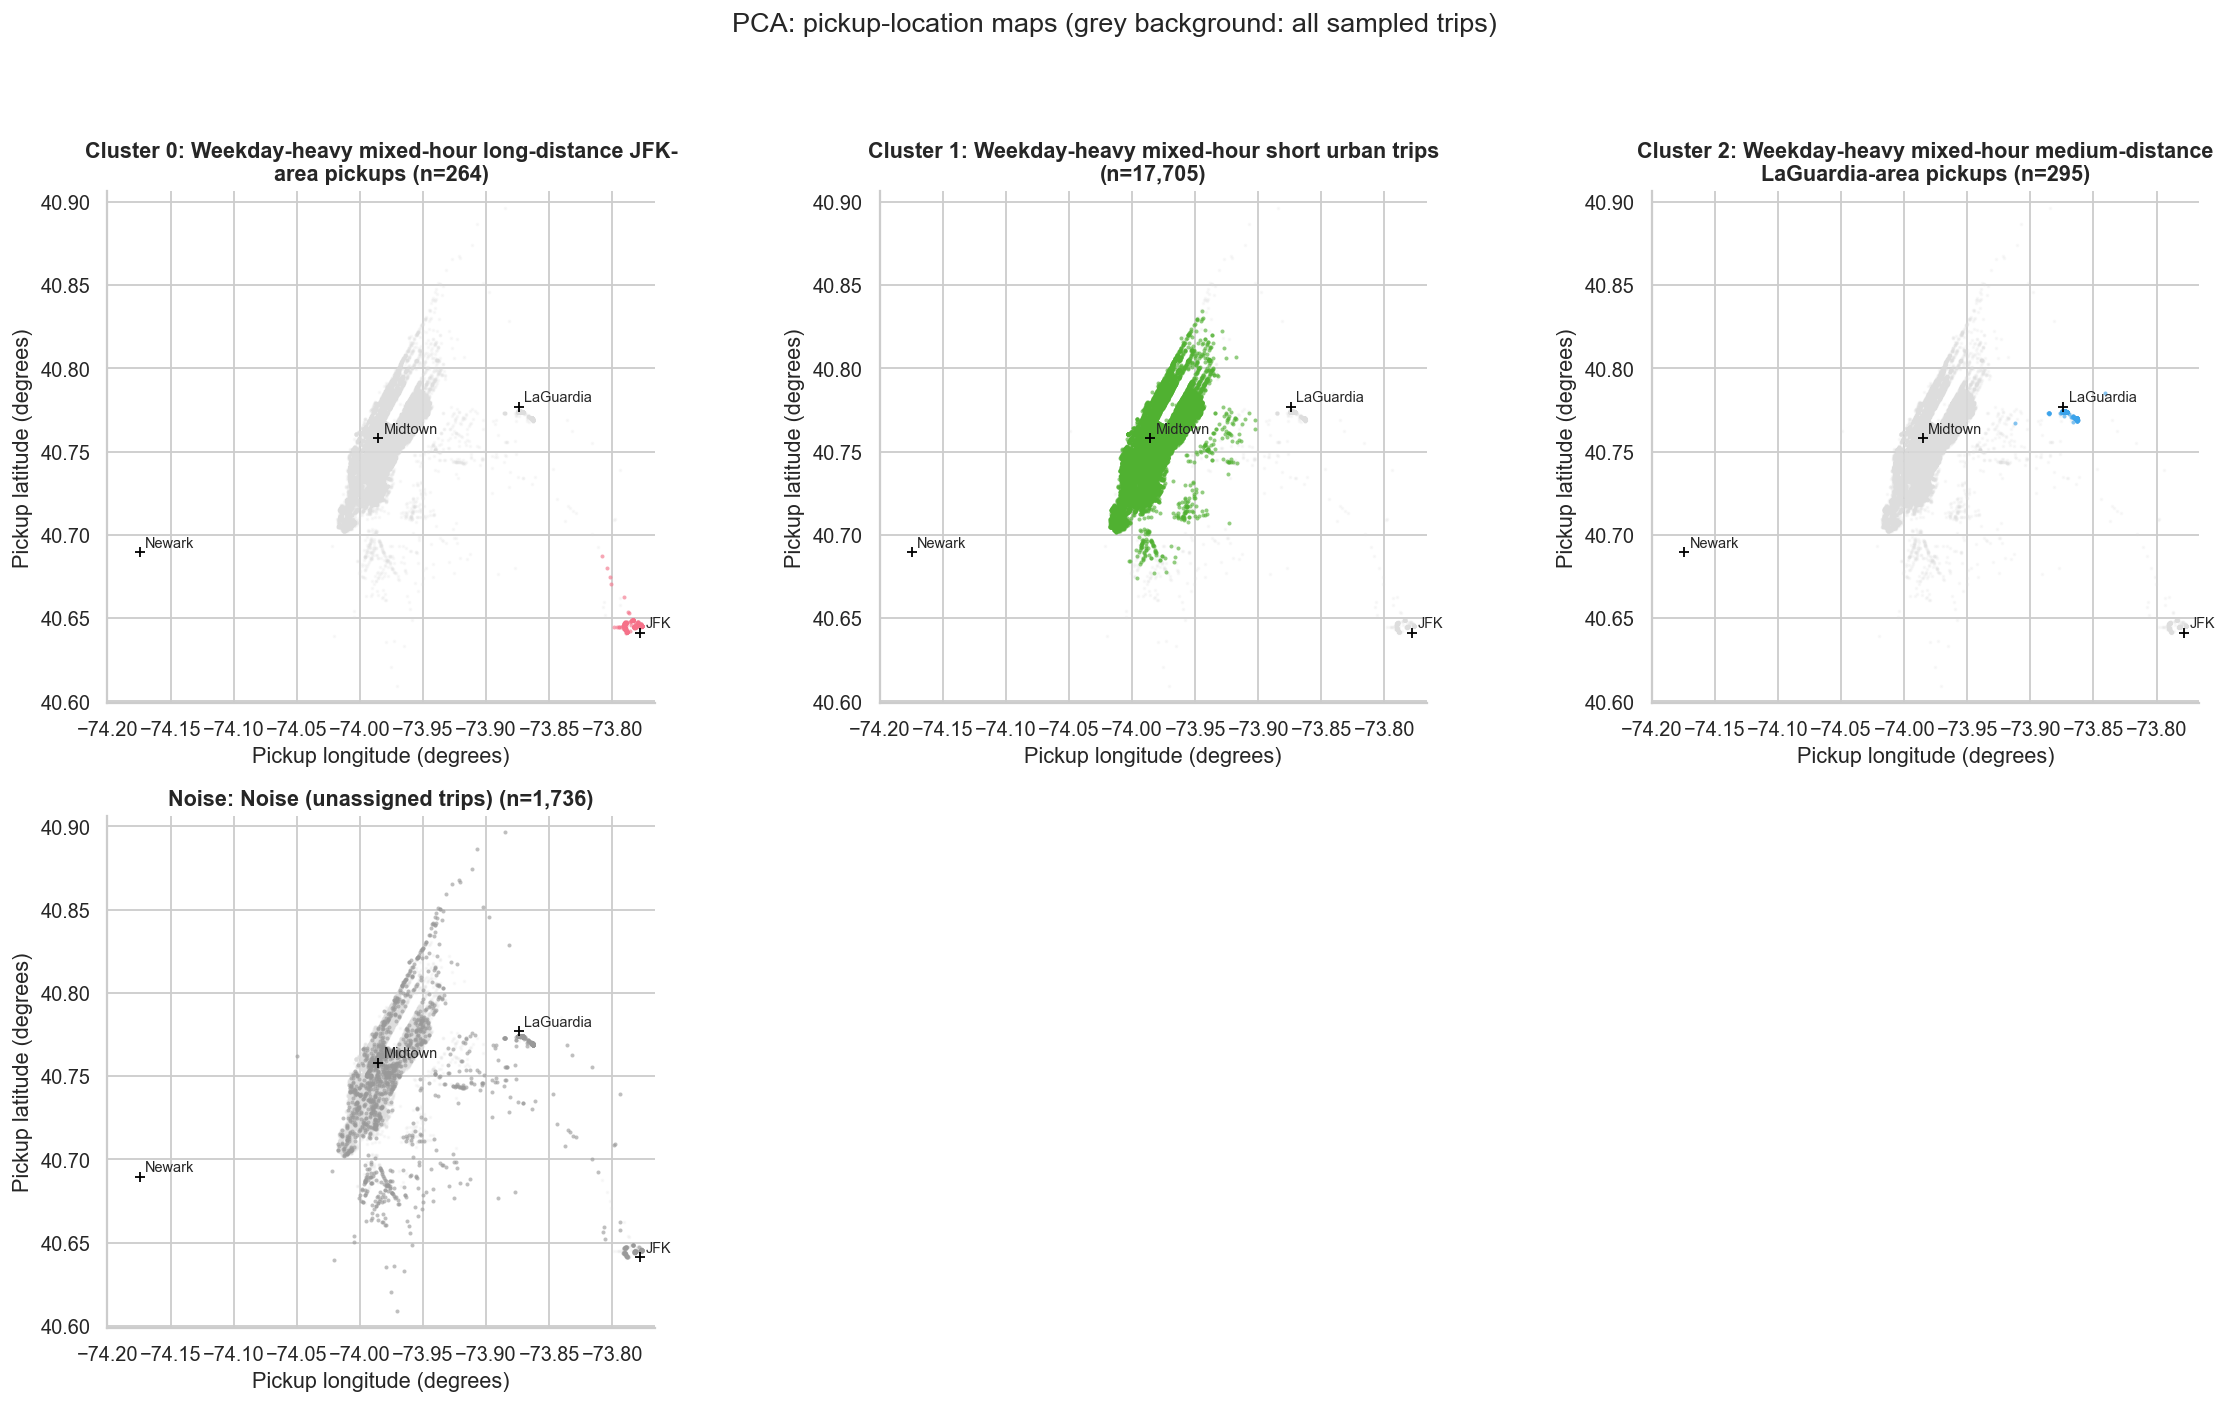
\includegraphics[width=\linewidth]{figures/clustering_pickups_pca.png}
  \caption{Pickup locations for each PCA-space cluster and noise.}
  \label{fig:cluster-pca-map}
\end{figure}

\begin{figure}[H]
  \centering
  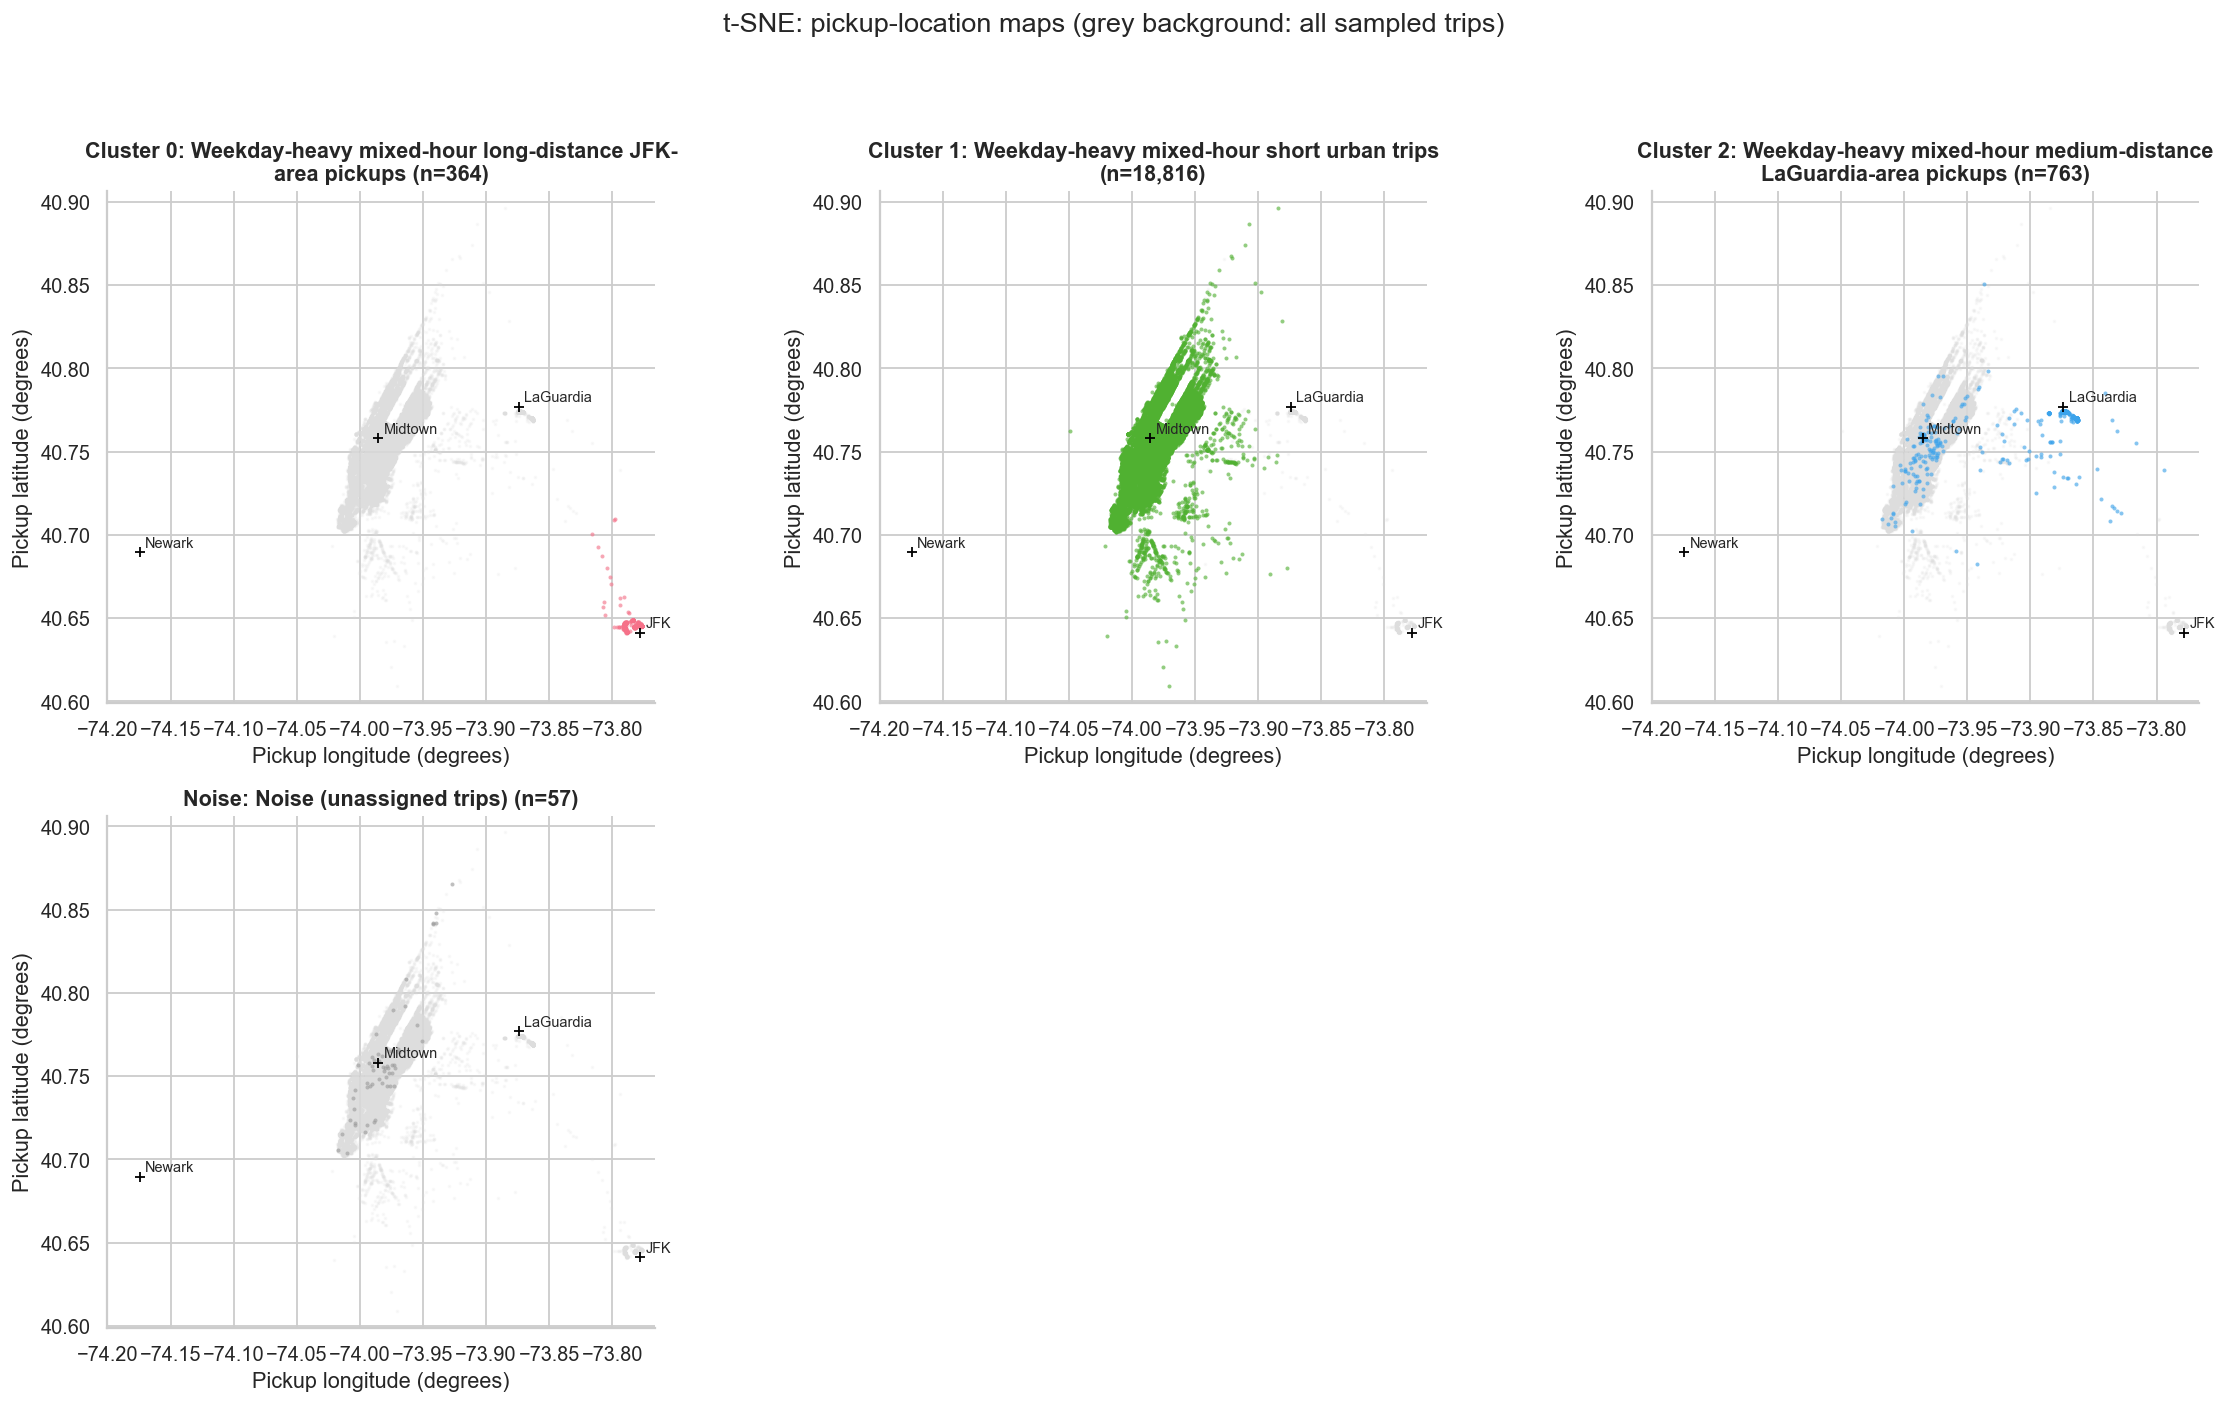
\includegraphics[width=\linewidth]{figures/clustering_pickups_tsne.png}
  \caption{Pickup locations for each t-SNE-space cluster and noise.}
  \label{fig:cluster-tsne-map}
\end{figure}

\begin{figure}[H]
  \centering
  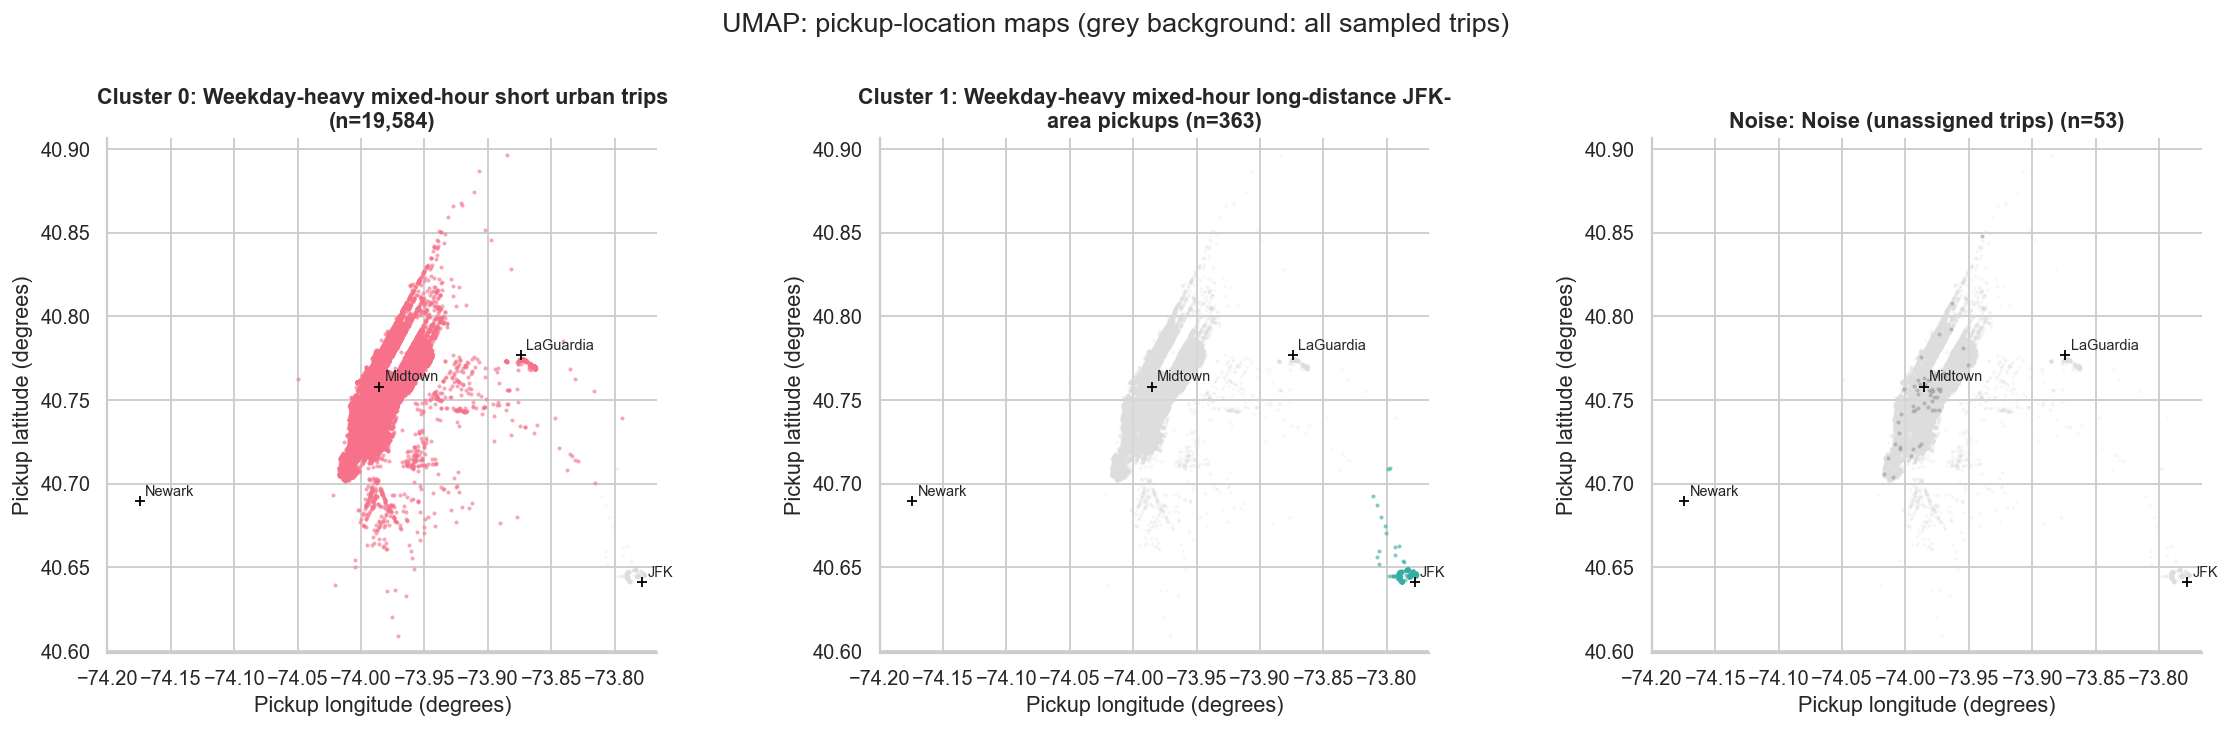
\includegraphics[width=\linewidth]{figures/clustering_pickups_umap.png}
  \caption{Pickup locations for each UMAP-space cluster and noise.}
  \label{fig:cluster-umap-map}
\end{figure}

Clustering t-SNE or UMAP measures density in a changed two-dimensional space,
not in the original features. Their low noise fractions do not prove better
clustering. The large urban groups contain many trip types, and visible
time-based lobes are not necessarily separate excess-of-mass clusters.
Noise means unassigned under these settings, not invalid data.
These are exploratory results. They depend on feature weights, the sample,
embedding settings and density parameters, especially for PCA.

\subsection{Comparison of PCA, t-SNE and UMAP}

Figure~\ref{fig:embedding-comparison} places the selected views side by side
with identical logarithmic distance colouring: PC1/PC2, t-SNE perplexity 30,
and UMAP with 15 neighbours and minimum distance 0.5. Every panel contains
the same 20,000 trips. Each method has its own coordinates and scale.
PCA clustering still uses nine components, not just the two displayed.

\begin{figure}[H]
  \centering
  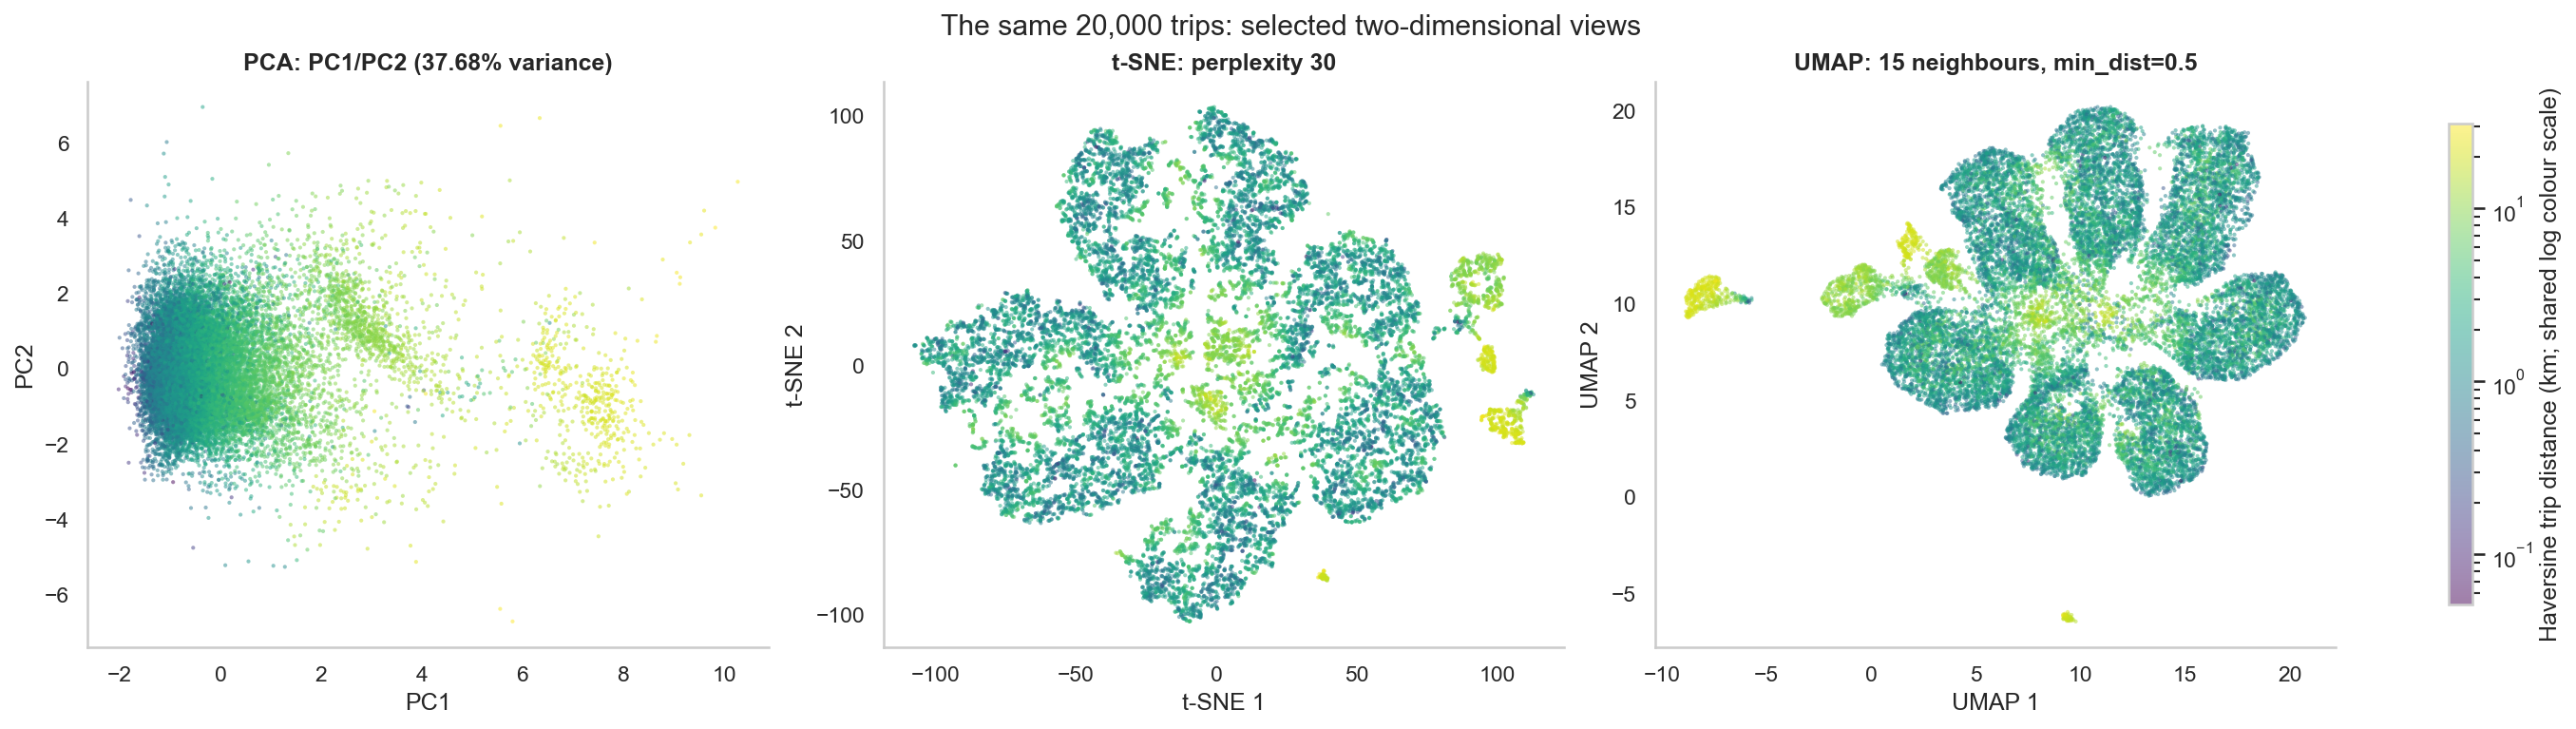
\includegraphics[width=\linewidth]{figures/embedding_comparison.png}
  \caption{Selected two-dimensional views with a common trip-distance colour
  scale. The log transform affects colour only.}
  \label{fig:embedding-comparison}
\end{figure}

\subsubsection{Consistent groups and the linear versus nonlinear views}

A large group of short urban trips and a group of long-distance JFK-area
pickups appear across all three methods. All 264 members of the PCA JFK group also
belong to the nonlinear JFK groups; the t-SNE and UMAP groups contain 364
and 363 trips, with 363 in common. Their approximately 20 km median
distances and original pickup-location maps support this description,
although proximity does not prove the reason for travel.
Not all airport groups remain separate: PCA and t-SNE identify
LaGuardia-area groups with 295 and 763 members (294 in common), whereas
UMAP includes these trips in its broad urban group. Group boundaries
therefore depend on the method.

PCA shows gradual changes in distance, duration and speed, plus a geographic
second axis. Its feature coefficients can be interpreted directly.
The 2D display retains only 37.68\% of variance, so overlapping points can
hide differences along later components. The nine components used for
clustering retain 94.58\%. Nonlinear views show lobes with similar hour and
weekday values that PCA's linear 2D view largely misses. However, the
selected HDBSCAN hierarchy does not treat every visible lobe as a separate cluster.

\subsubsection{Local and global structure}

Local structure was measured using mean 15-neighbour recall: the fraction
of each trip's original 15 nearest neighbours that remain neighbours after
reduction. This was averaged over 2,000 fixed random query trips, with
neighbours found among all 20,000 trips and the query itself excluded.
A rough measure of global structure was the Spearman correlation of distances
for the same 10,000 random pairs of distinct trips. Both checks use the
original standardized 11D space as a reference. They do not independently
validate groups or measure whether density is preserved.

\begin{table}[H]
  \caption{Observed structure preservation. PCA 9D is the clustering
  representation, not a fourth 2D plot.}
  \centering
  \begin{tabular}{lrr}
    \toprule
    Space & Mean 15-neighbour recall & Pair-distance Spearman \\
    \midrule
    PCA 2D & 0.0255 & 0.7486 \\
    t-SNE 2D & 0.5125 & 0.3120 \\
    UMAP 2D & 0.2345 & 0.3582 \\
    PCA 9D & 0.7877 & 0.9891 \\
    \bottomrule
  \end{tabular}
\end{table}

t-SNE best preserves immediate neighbours among the 2D views in this
experiment. UMAP does better than PCA 2D locally, but not better than t-SNE.
PCA best keeps the broad ordering of distances, particularly in 9D.
UMAP's pair-distance correlation is slightly higher than t-SNE's, but both
are low. This does not show that either gives accurate global geometry.

PCA uses orthogonal axes, so distances in the retained components cannot
exceed distances in the original standardized features. However, dropping
components can make distances much smaller. PCA does not minimize the
distance error for every pair. t-SNE optimizes local similarity probabilities,
while UMAP optimizes a fuzzy neighbourhood graph. Neither nonlinear map has
axes in physical-distance units or PCA-style feature loadings.
Gaps between islands, their order, area and apparent density do not reliably
describe the original feature space. Even PCA's plot area shows projected
spread, not the number of trips. Cluster sizes must be read from membership
counts, not visual area. None of these distances is a road distance.

\subsubsection{Runtime and sensitivity}

Repeat fits at seeds 42 and 43 were timed after earlier runs had warmed up
the software. Timings cover only
\texttt{fit\_transform}, excluding imports, preprocessing, clustering and
plotting. Numerical thread pools were limited to two, with one UMAP
optimization worker. All other settings matched the selected runs.

\begin{table}[H]
  \caption{Warm fit times and seed-to-seed cluster agreement. PCA uses full
  SVD; its seed is irrelevant. UMAP compilation overhead is excluded.}
  \centering
  \begin{tabular}{lrrr}
    \toprule
    Method & Seed 42 time (s) & Seed 43 time (s) & Cluster ARI \\
    \midrule
    PCA & 0.0043 & 0.0044 & 1.0000 \\
    t-SNE & 91.39 & 94.23 & 1.0000 \\
    UMAP & 16.60 & 16.44 & 1.0000 \\
    \bottomrule
  \end{tabular}
\end{table}

PCA is by far the fastest, and UMAP is about 5.5 times faster than t-SNE here.
Exact timings depend on hardware, software, system load, thread limits,
iteration budgets and first-use overhead. Full-SVD PCA gives repeatable
results but depends on feature scaling and the number of retained dimensions.
t-SNE depends on perplexity,
initialization, learning rate, iteration budget and seed. UMAP depends on
neighbourhood size, minimum distance, initialization, epochs and seed.
Earlier parameter tests visibly changed both nonlinear layouts and how
tightly their points were packed. All selected clusterings were identical
between seeds 42 and 43 and matched their earlier seed-42 labels.
This shows stable cluster assignments for those two runs only. It does not
show identical coordinates, stable neighbourhoods, convergence or stability
across other seeds.

\subsubsection{Cluster agreement and validity}

Adjusted Rand index (ARI) measures cluster agreement while adjusting for
chance. Changing cluster numbers does not affect it. ARI equals one for
identical clusterings, is near zero for chance-level agreement and can be
negative. Table~\ref{tab:ari-comparison} reports ARI for all trips, treating
-1 as a shared noise label, and for trips assigned to a non-noise cluster
by both methods. The second measure uses a different set of trips and
leaves out difficult cases.

\begin{table}[H]
  \caption{Pairwise cluster agreement. Noise handling is explicit.}
  \label{tab:ari-comparison}
  \centering
  \begin{tabular}{lrrr}
    \toprule
    Pair & ARI, all trips & Both assigned & ARI, shared assigned subset \\
    \midrule
    PCA--t-SNE & 0.6188 & 18,264 & 0.9905 \\
    PCA--UMAP & 0.2678 & 18,264 & 0.6311 \\
    t-SNE--UMAP & 0.5005 & 19,943 & 0.4686 \\
    \bottomrule
  \end{tabular}
\end{table}

\begin{figure}[H]
  \centering
  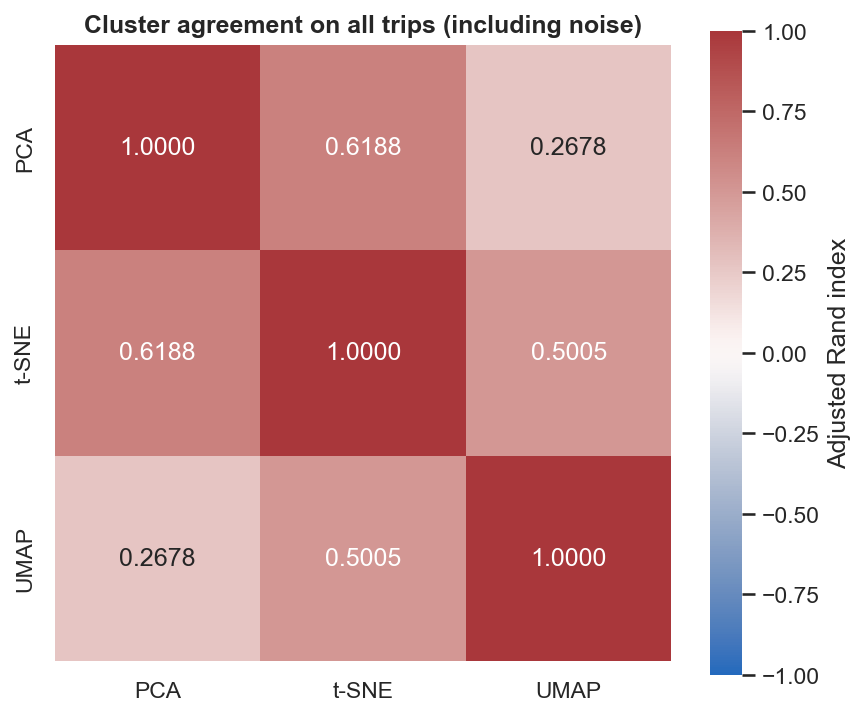
\includegraphics[width=0.65\linewidth]{figures/clustering_ari_comparison.png}
  \caption{ARI on all 20,000 trips, including noise.}
  \label{fig:ari-comparison}
\end{figure}

PCA and t-SNE agree most strongly overall. Of the 1,736 PCA noise trips,
t-SNE assigns 1,119 to its urban group, 460 to its LaGuardia group and
100 to its JFK group, leaving 57 as noise. Excluding unassigned cases
therefore increases their ARI sharply. UMAP merges all 763 t-SNE
LaGuardia-group trips into its urban group, despite recovering almost
the same JFK group. The notebook cross-tabulations show these differences.
A large shared urban group can hide disagreement about smaller groups.

Nonlinear clusters should be treated as possible groups, not confirmed trip
classes. t-SNE and UMAP change density, and HDBSCAN finds dense groups in
those changed spaces. Clear islands, low noise or agreement between methods
or seeds are not enough to confirm real groups. Original-unit profiles,
pickup maps and the JFK group found in nine-dimensional PCA give stronger
support. However, all methods use the same features and may share biases.
Further checks would need the full standardized feature space, new samples,
more seeds and density settings, and independent geographic or operational
evidence. This analysis does not claim independent validation.

\subsubsection{Recommendation}

Use \textbf{UMAP with 15 neighbours and minimum distance 0.5 as the primary
exploratory 2D map, paired with PCA as an interpretable reference}.
UMAP is much faster than t-SNE here, shows local time patterns and finds
the recurring JFK group without the tight packing caused by minimum
distance 0.0. Check apparent nonlinear groups against nine-dimensional
PCA and original-feature profiles and maps, rather than treating UMAP
density as ground truth. If keeping immediate neighbours is the main
priority, use t-SNE instead: it gave the best 2D neighbour recall in this
experiment. For broad geometry, feature interpretation or a repeatable
baseline, prefer PCA, but do not rely only on its two-dimensional display.

\section*{References}

\small

\begin{thebibliography}{1}
\bibitem{nyctaxi}
Kaggle. \emph{New York City Taxi Trip Duration}.
\url{https://www.kaggle.com/c/nyc-taxi-trip-duration}.
\end{thebibliography}

\end{document}
